%% Survey + proposal + implementation + examples for connecting EXHALE to the
%% lower atmosphere.  Companion of lower_atmosphere_coupling.md.
\documentclass[english,a4paper]{my_memo}
\usepackage{booktabs}
\usepackage{graphicx}
\graphicspath{{lower_atmosphere_figs/}}

\newcommand{\Rp}{R_{\mathrm{p}}}
\newcommand{\RJ}{R_{\mathrm{J}}}
\newcommand{\Mdot}{\dot{M}}
\newcommand{\ubar}{\mu\mathrm{bar}}
\newcommand{\qHH}{q_{\mathrm{H_2}}}

\title{Connecting EXHALE to the Lower Atmosphere:\\ Survey, Implementation, and Example Applications}
\author{Kwang-Il Seon}
\date{Last updated: 2026-08-19}

\begin{document}
\maketitle

\section{Motivation and current state}

EXHALE's lower boundary is the $\sim$1\,$\ubar$ level: the input ``Planet radius'' is the
\emph{radius of that level} (user-guessed), the base temperature is fixed at
$T_0=T_\mathrm{eq}$, the base density $n_0$ is an input (or pressure-anchored via
\texttt{base\_p\_ubar}), and the gas is purely atomic H/He $+$ trace metals at prescribed
abundances. No molecules exist anywhere in the domain. The Wind-AE IC port carries a
\emph{simplified} molecular layer ($\mu$-blend \texttt{molec\_adjust} $+$ bolometric
heating/cooling, auto-shutoff when the atomic transition reaches the base).

\emph{[2026-08-15: this paragraph describes the tree as of 2026-07 and is no
longer current. The coupled molecular network (H$_2$/H$_2^+$/H$_3^+$/HeH$^+$,
\texttt{Molecular chemistry: True}), H$_3^+$ cooling, Lyman--Werner
photodissociation, the analytic lower column and the \texttt{base.inp} handoff
are all implemented in \texttt{src/modules/lower\_atmosphere/}. They default
off, so an ordinary run is still the atomic base described here; the status table
of each tier is the authoritative account.]}

This memo (i) surveys how the literature connects escape models to the lower atmosphere,
(ii) documents the implementation in \texttt{src/modules/lower\_atmosphere/} and
\texttt{src/utils/run\_lower.py}, (iii) applies it to the four planets modeled with
EXHALE (HD\,209458\,b, HD\,189733\,b, WASP-121\,b, WASP-52\,b), and (iv) prescribes how
the outputs are used and connected to EXHALE runs.

\section{What the literature does at the interface}

\begin{table}[h]\centering\small
\begin{tabular}{@{}p{2.5cm}p{4.2cm}p{4.4cm}p{3.6cm}@{}}
\toprule
Approach & Lower atmosphere & Hands to the wind model at $\sim$1\,$\ubar$ & Cost / availability \\
\midrule
Salz et al.\ (2016), TPCI & none: CLOUDY solves the whole column (molecules disabled) &
  n/a (single domain; base at $n=10^{14}$\,cm$^{-3}$, $T_\mathrm{eq}$) &
  $\sim$$3\times10^{5}$ CPU-h for 18 planets; interface not public \\
Koskinen et al.\ (2022) & \emph{analytic}: isothermal-$T_\mathrm{eq}$ hypsometric column from
  1 bar, $\mu(p)$ from chemical-equilibrium H$_2$/H/He fits (Visscher et al.\ 2006) &
  base \emph{radius} $r_0$(1\,$\ubar$), $T_0{=}T_\mathrm{eq}$, $\qHH/q_\mathrm{H}/q_\mathrm{He}$;
  base $v$ from mass conservation & trivial (closed-form; all equations in the paper) \\
Huang et al.\ (2017) & \emph{analytic spacer}: isothermal $\mu{=}2.3$ column, 1 bar $\to$ 10\,$\ubar$ &
  base radius of the atomic layer; Ly$\alpha$ \emph{absorbing} bottom boundary
  (H$_2$ accidental resonances, $\tau{=}1$ at $N_\mathrm{H_2}{\approx}10^{14}$\,cm$^{-2}$) & trivial \\
Taylor et al.\ (2025, 2026) & full Lavvas \& Arfaux (2021) model (RC temperature $+$
  $\sim$150-species kinetics of Lavvas et al.\ 2014 $+$ haze microphysics;
  $10^{3}\to10^{-6}$ bar) & $T$(1\,$\ubar$), altitude of the 1\,$\ubar$ level, composition
  (with a \emph{tolerated discontinuity}), $K_{zz}$ & in-house, \textbf{not public};
  coupling is a manual splice, iterated $\sim$3$\times$ \\
\bottomrule
\end{tabular}
\end{table}

\noindent Key quantitative facts:
\begin{itemize}
\item \textbf{Base insensitivity for strong winds} (Salz et al.\ 2016, \S3.5--3.6):
  $T_\mathrm{base}\pm40\% \Rightarrow \Mdot\pm5$--$10\%$ (linear); base density
  $10^{14}\to10^{12}$\,cm$^{-3}$ $\Rightarrow \Mdot\lesssim40\%$ lower. Their error budget:
  base density $\pm50\%$, base $T$ $\pm10\%$, both dwarfed by the XUV uncertainty
  ($\times3$). $\Rightarrow$ \emph{EXHALE's fixed-$T_\mathrm{eq}$ base is already
  defensible for hot Jupiters.}
\item \textbf{Where the fixed base breaks:} (i) planets near radiative equilibrium
  (stable thermospheres); (ii) cool/sub-Neptune planets where H$_2$ survives into the
  wind, Salz's GJ\,1214\,b test: H$_2$ 10--25\% throughout, H$^-$ a significant coolant,
  $\Mdot-15\%$; Taylor et al.\ (2026): adding H$_2$ \emph{halves} the He 10830 signal
  (14\%$\to$7\%); Koskinen et al.\ (2022) hot Uranus: base $\qHH\approx0.84$ and H$_3^+$ IR
  emission is the dominant radiative coolant below $\sim$2.3\,$\Rp$.
\item \textbf{What a photochemical lower model uniquely provides} (Lavvas et al.\ 2014;
  Lavvas \& Arfaux 2021): the H$_2\to$H transition can sit exactly at 1\,$\ubar$ and is
  temperature-sensitive there; photochemistry (OH-catalyzed H$_2$ destruction) dissociates
  H$_2$ even at 500--1000\,K; \emph{atomic-metal release profiles} (Na, K, Mg, Ca, Fe, Al,
  Si return to atomic form below $\sim$$10^{-3}$ bar), the physically-motivated base
  abundances for EXHALE's trace metals; photoionization-dominated electron density
  ($\sim$$10^{8}$\,cm$^{-3}$, 100$\times$ Saha); radical/haze heating of $\pm$100--400\,K
  right at the handoff level. \emph{(2026-08-19: EXHALE carries no O/OH/H$_2$O
  species of its own, so this chemistry reaches the code only through the
  handoff. The directions open to us, with their costs and validation gates, are
  in \texttt{docs/oxygen\_chemistry\_options.md}.)}
\item \textbf{The published coupling is loose, not monolithic:} Lavvas et al.\ (2014) take
  $T(p<1\,\ubar)$ \emph{from} the Koskinen thermosphere and use ``species $<3$ amu escape
  at the wind velocity'' as their upper BC; Taylor et al.\ tolerate a composition
  discontinuity at 1\,$\ubar$. Only TPCI runs a tight coupling at every timestep (and it
  disables molecules).
\end{itemize}

\section{The three-tier plan}

\textbf{Tier 1}: analytic lower column (Koskinen-2022 style), deriving the 1-$\ubar$ base
radius and base H$_2$/H/He from a closed-form column. \textbf{Tier 2}: molecular
extension of EXHALE (H$_2$, H$_2^+$, H$_3^+$, HeH$^+$ chemistry $+$ H$_3^+$ IR cooling),
required only for warm Neptunes / sub-Neptunes; \textbf{Tier 2a}: an interim EOS-only
molecular-base correction. \textbf{Tier 3}: consume a real lower-atmosphere model
(photochemistry $+$ radiative--convective $T(p)$) through a file interface; the
open-source \texttt{VULCAN} (Tsai et al.\ 2017, 2021) $+$ \texttt{HELIOS} (Malik et al.\
2017) stack is the practical replacement for the non-public Lavvas \& Arfaux code, and a
TPCI-style full coupling is rejected (cost, availability, and demonstrated base
insensitivity). Which science case needs which tier: hot Jupiters $\to$ Tier 1 only;
He\,10830/H$\alpha$ work $\to$ Tier 1; metal transmission lines $\to$ Tier 3 (atomic-metal
release abundances); warm Neptunes / sub-Neptunes $\to$ Tier 2 $+$ 1.

% ===================================================================== %
\section{Implementation}\label{sec:impl}
% ===================================================================== %

All Fortran lives in \texttt{src/modules/lower\_atmosphere/}; the Python driver in
\texttt{src/utils/}. Everything is \textbf{opt-in / default off}: with no keys and no
\texttt{base.inp}, standard runs are unchanged by the lower-atmosphere code (the
molecular chemistry off-switch reproduces the atomic systems byte-for-byte; the
absolute production baseline itself moved with the 2026-07-23 defaults: staged
secondary ionization, \texttt{He\_rec\_coupling}, He--H charge exchange).

\subsection{Tier 1: \texttt{lower\_column.f90}}\label{sub:t1}

\paragraph{Equations.} The isothermal hypsometric relation is integrated from the 1-bar
level (radius $R_\mathrm{1bar}$, in practice the broadband transit radius) to the base
pressure $p_0=1\,\ubar$,
\begin{equation}
  \frac{\mathrm{d}\ln p}{\mathrm{d}r} \;=\; -\,\frac{\mu(p,T)\,m_\mathrm{H}\,g(r)}{k_\mathrm{B}T},
  \qquad g(r)=\frac{GM_\mathrm{p}}{r^{2}},\quad T=T_\mathrm{eq},
  \label{eq:hypso}
\end{equation}
with a fixed-step 4th-order Runge--Kutta in $x=\ln p$ (2000 steps; the integrand is
smooth). The mean molecular weight follows the chemical-equilibrium H$_2$/H partition of
Visscher et al.\ (2006) as fitted by Koskinen et al.\ (2022, Eq.~11),
\begin{equation}
  \qHH \simeq \frac{1.9845 + 10^{u} - \sqrt{10^{u}\,(3.9690 + 10^{u})}}{2.3670},
  \qquad u = -\frac{23672}{T} - \log_{10} p_\mathrm{[bar]} + 6.2645 .
  \label{eq:visscher}
\end{equation}
An implementation subtlety uncovered during validation: Eq.~\eqref{eq:visscher} returns
the \emph{full-mixture} volume mixing ratio $\qHH = n_\mathrm{H_2}/(n_\mathrm{H_2}+
n_\mathrm{H}+n_\mathrm{He})$ (a protosolar He abundance is baked into the fit), so the
fraction $x_2$ of H \emph{nuclei} bound in H$_2$ must be recovered as
\begin{equation}
  x_2 \;=\; \frac{2\,\qHH\,(1+f_\mathrm{He})}{1+\qHH}\;\le\;1,
  \qquad
  \mu \;=\; \frac{1+4f_\mathrm{He}}{(1-x_2)+x_2/2+f_\mathrm{He}}\;\;[\mathrm{amu}],
  \label{eq:x2}
\end{equation}
with $f_\mathrm{He}=n_\mathrm{He}/n_\mathrm{H(nuclei)}$ the elemental ratio (EXHALE's
\texttt{HeH}). Equation~\eqref{eq:x2} was verified against the Koskinen et al.\ (2022)
Model~A base composition ($\qHH=0.84$, $q_\mathrm{H}=0.026 \Rightarrow x_2=0.985$); the
naive H-subsystem inversion $x_2=2q/(1+q)$ is \emph{wrong} and misses the gate.

\paragraph{Interface.} \texttt{lower\_column\_solve(Mp, R\_deep, T, fhe, p\_deep, p\_base,
r\_base, qh2\_b, qh\_b, qhe\_b, mu\_b, r\_base\_atomic)} (cgs; pressures in bar). Because
chemical equilibrium \emph{underestimates} H dissociation at
$T_\mathrm{eq}\approx1000$--2000\,K (photochemistry ignored; Moses et al.\ 2011; Koskinen
et al.\ 2013a), the routine also integrates the same column with the fully atomic
$\mu=(1+4f_\mathrm{He})/(1+f_\mathrm{He})$ and returns \texttt{r\_base\_atomic}: the two
radii \emph{bracket} the truth. The public helper \texttt{q\_h2\_equilibrium(p,T)} exposes
Eq.~\eqref{eq:visscher} (NaN-safe, clamped to $[0,1]$).

\paragraph{EXHALE key.} \texttt{Lower column: <R\_1bar in R\_J>} in \texttt{input.inp}
triggers a startup report: the derived $r_0$(1\,$\ubar$) (equilibrium $+$ atomic bracket),
the input ``Planet radius'' for comparison, and the base $\qHH/q_\mathrm{H}/q_\mathrm{He}/\mu$,
plus a warning when the equilibrium base is strongly molecular. \emph{Report only:
nothing is overridden} (overriding is Tier 3's job, \S\ref{sub:t3}).

\paragraph{Validation gate (passed).} Koskinen et al.\ (2022) Model~A (Uranus-mass planet,
$M=8.6813\times10^{28}$\,g, $R_\mathrm{1bar}=2.5559\times10^{9}$\,cm, Sun-like star at
0.05\,au, $T_\mathrm{eq}=1140$\,K, $f_\mathrm{He}=0.0793$):
\begin{center}\small
\begin{tabular}{@{}lccc@{}}
\toprule
 & $r_0/R_\mathrm{1bar}$ & $\qHH$(base) & $q_\mathrm{H}$(base) \\
\midrule
this module & 1.343 & 0.838 & 0.027 \\
Koskinen et al.\ (2022) & 1.34 & $\approx$0.84 & $\approx$0.026 \\
\bottomrule
\end{tabular}
\end{center}
Approximations (documented in the source): isothermal column at $T_\mathrm{eq}$;
spherical gravity (the Roche-equipotential correction matters only near RLO); chemical
equilibrium only.

\subsection{Tier 2a: the \texttt{Molecular base} key}\label{sub:t2a}

\texttt{Molecular base: True} applies an \emph{EOS-only} correction at startup: the H
nuclei bound into H$_2$ at $(1\,\ubar, T_0)$ per Eq.~\eqref{eq:visscher}--\eqref{eq:x2}
are removed from the base particle budget,
\begin{equation}
  \mathtt{ntot\_bc} \;\to\; \mathtt{ntot\_bc} - \frac{x_2/2}{1+f_\mathrm{He}},
\end{equation}
which lowers the base pressure ($p_\mathrm{base}= \mathtt{ntot\_bc}\,n_0 k_\mathrm{B}T_0$)
and raises the base mean molecular weight, i.e.\ a heavier, more compact base, the
leading-order effect of a molecular base on the hydrodynamics. The species arrays remain
atomic (H$_2$ chemistry is Tier-2 proper), so this is a \emph{crude, clearly-flagged}
approximation. \emph{[2026-08-15: \texttt{Molecular chemistry: True} turns this
key on by itself (an atomic \texttt{ntot\_bc} beneath a molecular base is
physically inconsistent), so it need not be set separately for a Tier-2 run.]} Example: HD\,209458\,b, $\qHH(1\,\ubar,1450\,\mathrm{K})=0.831
\Rightarrow \mathtt{ntot\_bc}\,1.0\to0.546$.

\subsection{Tier 2 foundation: \texttt{h3p\_cooling.f90} and \texttt{mol\_rates.f90}}\label{sub:t2}

\paragraph{H$_3^+$ infrared cooling.} Optically thin cooling per molecule from Miller et
al.\ (2013, Table~5, $z(T)$ fits, archived as
\texttt{references/Miller\_2013\_JPCA\_117\_9770.pdf}):
\begin{equation}
  \ln E(\mathrm{H_3^+},T) = \sum_n C_n T^{\,n}
  \qquad [E\ \mathrm{in\ W\,molecule^{-1}\,sr^{-1}}],
\end{equation}
piecewise over 30--300, 300--800, 800--1800, and 1800--5000\,K (fit errors $<0.1\%$ over
300--5000\,K), held frozen above 5000\,K (H$_3^+$ is destroyed well below). The
volumetric rate is
\begin{equation}
  \Lambda_{\mathrm{H_3^+}} = n_{\mathrm{H_3^+}}\;4\pi\,E(T)\;
  s_\mathrm{nonLTE}(T,n_{\mathrm{H_2}})\times10^{7}
  \quad[\mathrm{erg\,s^{-1}\,cm^{-3}}],
\end{equation}
where $s_\mathrm{nonLTE}$ is the departure factor of Miller et al.\ (2013, Table~6; their
Oka \& Epp detailed-balance approach), implemented as a bilinear interpolation in
$(T,\log_{10}n_\mathrm{H_2})$ over $T=300$--5000\,K and $n_\mathrm{H_2}=10^{6}$--$10^{14}$
cm$^{-3}$; $s\to1$ (LTE) at high density, and the tabulated values are upper limits per
the paper's caveat on the proton-hopping rate. Both interpolators use the NaN-safe
\texttt{.not.(x>edge)} bracketing adopted after the 2026-07-02 code review.
\textbf{Validation:} the fits reproduce the paper's Table-4 anchors at
$T=500/1000/2000/3000/5000$\,K to $<$0.5\%, and $s(1000\,\mathrm{K},10^{10}\,
\mathrm{cm^{-3}})=0.4955$, $s(2000\,\mathrm{K},10^{12})=0.9499$ exactly.

\paragraph{Molecular reaction rates.} \texttt{mol\_rates.f90} provides the full
H$_2$/H$_2^+$/H$_3^+$/HeH$^+$ thermochemical network of Koskinen et al.\ (2022, Table~1;
transcribed and verified against the PDF page): recombination (R1--R2, Storey \& Hummer
1995), Voronov (1997) collisional ionization (R3--R4), H$_2^+$/H$_3^+$/HeH$^+$
dissociative recombination (R5--R7, R16; Larsson et al.\ 2008), the H$_3^+$ production
backbone H$_2^+ + \mathrm{H_2}\to \mathrm{H_3^+} + \mathrm{H}$ (R8, $2\times10^{-9}$),
thermal and electron-impact H$_2$ dissociation (R12, R14), three-body chemistry (R13,
R15), the HeH$^+$ chain (R17--R20), and H/He charge exchange (R21--R23). The stellar
photo-rates P1--P5 (including H$_2$ dissociative and double photoionization) follow
EXHALE's existing \texttt{PH\_heat} routines once H$_2$ cross sections are added.
Lyman--Werner neutral photodissociation is not part of the source network
(Koskinen et al.'s sensitivity test bounded its effect on $\Mdot$ at
$\times1.4$); EXHALE adds it separately and opt-in, keyed on the band flux at
the planet (\texttt{Stellar LW flux}, 2026-08-13, \S\ref{sec:lw}).

\paragraph{Tier-2 core (implemented 2026-07-03).} The coupled system
\texttt{System\_HeH\_mol.f90} solves 7--8 unknowns per cell (H$^+$, He$^+$, He$^{++}$,
optionally He\,2$^3$S, plus the H-nucleus fractions bound in H$_2$, H$_2^+$, H$_3^+$,
HeH$^+$) as element-conserving steady-state balances with \texttt{hybrd1}: the atomic
rows use EXHALE's own rate arrays (so the molecule-free limit reproduces the atomic
systems' solution) and the molecular channels are the Table-1 network via
\texttt{mol\_rates} (R21/R22 H--He charge exchange deliberately excluded to preserve
the atomic limit). The H$_2$ photoionization cross section (Yan et al.\ 1998,
Eqs.~17--19; verified against their Table~7 to $<$0.2\%) enters the opacity, the P$_{\rm H_2}$
photoionization integral, the photoelectric heating, and the absorbed-energy
normalization through optional arguments of \texttt{PH\_heat\_HHe}; H$_3^+$ IR cooling
enters the \texttt{cool} array. The EOS counts each molecule as one particle, each
molecular ion's electron, and the correct masses (\texttt{calc\_ne/ntot/rho},
\texttt{get\_species\_densities}). \texttt{f\_sp} grows to 37 columns (output schema
and Load-IC names extended). Key: \texttt{Molecular chemistry: True} (requires He; v1
excludes trace metals; the molecular base particle count is coupled on automatically,
an atomic \texttt{ntot\_bc} under a molecular base is physically inconsistent).
\textbf{Gates passed} (numbers re-established 2026-07-16 after the deterministic
chemical-equilibrium seeding of the molecular solve; the exact gate inputs are pinned at
\texttt{lower\_atmosphere\_figs/data\_g*/input.inp}): (0) molecules-off regression,
molecular chemistry off reproduces the atomic systems; (1) HD\,209458\,b molecules-on: a
fully molecular base ($x_{\rm H_2}\simeq0.996$) with a sharp H$_2\to$H front at
$r=1.020\,\Rp$ and an essentially atomic wind above it (the hot-Jupiter atomic base
is now a \emph{result}, not an assumption), while below the front the molecular base
suppresses He\,2$^3$S by orders of magnitude (He\,2$^3$S$+$H$_2$ Penning destruction,
${\sim}10^4\times$ at the front, rising back to the atomic value above ${\sim}1.3\,\Rp$);
(2) a hot-Uranus-like case (0.0457\,$M_{\rm J}$, $R_{\rm p}=0.49\,R_{\rm J}$,
$T_{\rm eq}{=}1140$\,K, HD\,209458\,b orbit and spectrum): the front sits at
$r=1.156\,\Rp$ and H$_3^+$ is active below it (peak ${\sim}7{\times}10^4$\,cm$^{-3}$ at
$r{\approx}1.04$). The H$_2\to$H fronts and molecular base composition are essentially
unchanged from the 2026-07-16 gates (front $1.019{\to}1.020$, $1.166{\to}1.156$),
confirming the dissociation-front result is robust to the 2026-07-23 production defaults;
refreshed 2026-07-23 at a shared 12000-step relaxation-snapshot convention (both HD209
runs $\log\Mdot=10.58$; relaxation snapshots, not flux-flat converged).
Figure~\ref{fig:mol} shows the gate runs. Both gate configurations were
Newton-converged on 2026-08-13 once the H$_3^+$ cooling entered the marching
energy update; the converged solutions differ substantially from these
snapshots below the H$_2\to$H front and are given in \S\ref{sec:converged}.

\paragraph{He\,2$^3$S $+$ H$_2$ Penning ionization.} When \texttt{Include
He23S?} is also on, the metastable couples to H$_2$ through Penning ionization
He($2^3$S)$+$H$_2\to$He($1^1$S)$+$H$_2^+ + e^-$: the dominant He($2^3$S) loss
toward an H$_2$-dominated base (Garc\'ia Mu\~noz 2025, A\&A 698, A199, Fig.~4).
Its rate coefficient \texttt{penning\_HeI23S\_H2} (\texttt{Cool\_coeff.f90}) is
an analytic fit to Garc\'ia Mu\~noz Table~A.5 (Cohen \& Lane 1977 cross
sections), $k(T)=5.3791\times10^{-12}\,T^{0.6760}\,e^{-695.21/T}\,
\mathrm{cm^3\,s^{-1}}$, reproducing the tabulated 500--10000\,K points to
$\le0.13\%$. It enters \texttt{System\_HeH\_mol} as an H$_2$ loss / H$_2^+$
source / He($2^3$S) sink and adds $(E[2^3S]-\mathrm{IP}[\mathrm{H_2}])\approx
4.4\,$eV of electron heating; the minor associative H$+$HeH$^+$ branch
(${\sim}10\%$) is folded into the Penning channel.

\paragraph{The \texttt{\_adv} post-process is atomic-only, so the Penning-H$_2$
term does not appear there.} The advection-corrected reconstruction in
\texttt{post\_process\_adv.f90} (header, lines 4--13) treats the gas as
H/He\,$+$\,trace metals and excludes the molecular species entirely: the
molecular densities are never passed in or re-solved, and its
\texttt{calc\_ne}/\texttt{calc\_ntot} calls omit the \texttt{nmol} argument.
Consequences for a molecular run: (i) the \texttt{\_adv} $n_{\rm tot}/n_e$ omit
the neutral-H$_2$ particle count and the molecular-ion electrons; (ii) the
He($2^3$S)$+$H$_2$ Penning sink cannot act in the \texttt{\_adv} solve (no
$n_{\rm H_2}$ there), so the \texttt{\_adv} outputs, and the transit module
that reads them, carry the \emph{equilibrium} molecular-base triplet
suppression ($39\times$ at the HD\,209458\,b base, $430\times$ on the
hot-Uranus case) without an advection correction. This is acceptable where
\texttt{\_adv} is physically meaningful (the atomic/ionized escape flow above
the H$_2\to$H front); below the front the atomic \texttt{\_adv} approximation
is outside its validity domain anyway. A molecular-aware \texttt{\_adv} is a
separate extension, naturally paired with the open ``molecular advection''
item in the Tier-2 remaining list.

\begin{figure}[htb]\centering
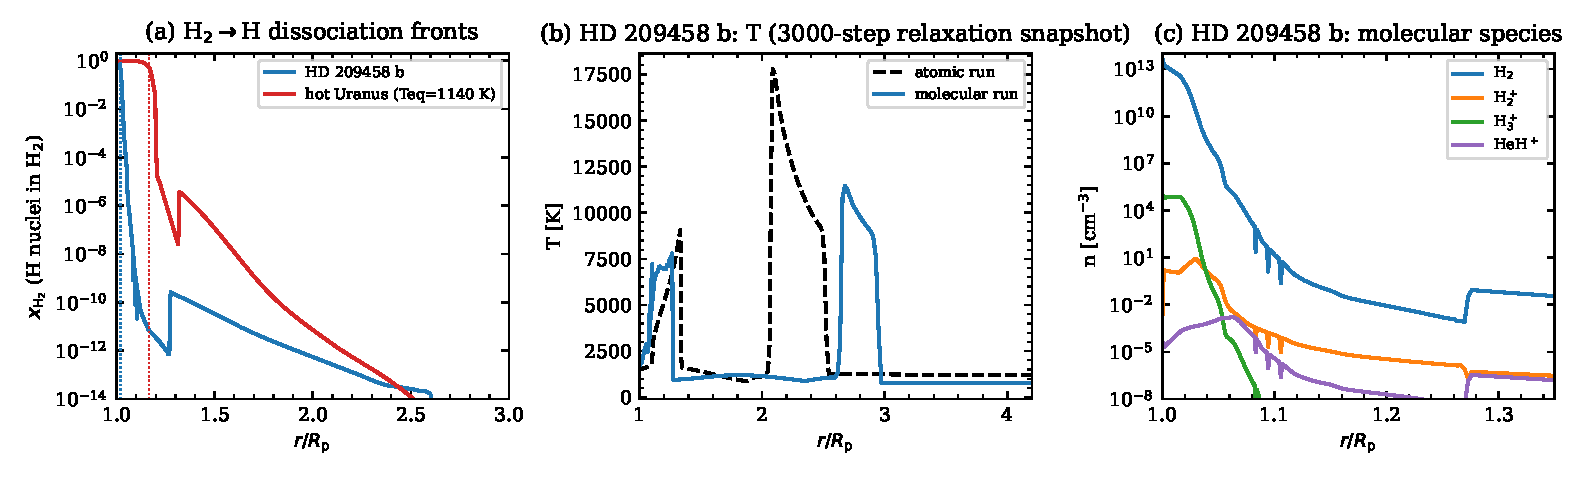
\includegraphics[width=\textwidth]{fig_mol_structure.pdf}
\caption{Tier-2 molecular gates (12000-step relaxation snapshots). (a) The H nuclei
fraction bound in H$_2$: on HD\,209458\,b the base is fully molecular and a sharp
H$_2\to$H front sits at $r=1.020\,\Rp$ (dotted); on the cooler, low-gravity hot
Uranus the front sits at $1.156\,\Rp$. The cell-to-cell flip-flop just above the
front marks the chemically bistable zone of \emph{equilibrium} H$_2$ chemistry:
kinetics$+$advection smooth it (the documented Tier-2 caveat). (b) The molecular run's
temperature agrees with the atomic run away from the (still-relaxing) front region.
(c) Molecular species on HD\,209458\,b: H$_3^+$ (green) and the molecular ions are
confined below the front, as expected for a hot Jupiter.}
\label{fig:mol}
\end{figure}

\paragraph{Trace metals in the same system (2026-08-13).} The molecular network and
the metal ionization stages are solved together in \texttt{System\_HeH\_mol\_metals},
so a \texttt{metals.inp} may sit in a molecular run. They cannot be solved apart:
in the shielded molecular base the metals are the dominant electron donors, and the
free electron density is shared by both sets of rows.

\paragraph{Remaining Tier-2 work (open).} Molecular \emph{advection} (the local
chemical-equilibrium treatment cannot reproduce Koskinen et al.'s advective
replenishment of high-altitude H$_2$ on cool Neptunes); the dissociative/double
photoionization channels (P4/P5); the 4.48\,eV dissociation energy sink of the
\emph{thermal} channels R12/R14; a diatomic $\gamma$; a molecule-aware
\texttt{\_adv} post-process; and the GJ\,1214\,b He-halving validation
(Taylor et al.\ 2026) with a full M-dwarf setup. Lyman--Werner photodissociation
(\S\ref{sec:lw}) and the metals$+$molecules merge left this list on 2026-08-13.

\subsection{Tier 3: \texttt{base.inp} and \texttt{run\_lower.py}}\label{sub:t3}

\paragraph{The handoff file.} An optional \texttt{base.inp} in the run directory is read
by \texttt{input\_read} \emph{before} the derived constants, so its overrides propagate
consistently ($v_0$, $b_0$, grid, normalization):
\begin{center}\small
\begin{tabular}{@{}llll@{}}
\toprule
key & unit & overrides & used by \\
\midrule
\texttt{T\_base}   & K     & $T_0$ (base temperature)          & thermal BC, EOS scales \\
\texttt{r\_base}   & $\RJ$ & ``Planet radius'' ($=r_0$ of 1\,$\ubar$) & grid, gravity, areas \\
\texttt{HeH\_base} & -     & He/H number ratio                 & composition, He diffusion \\
\texttt{Kzz\_base} & cm$^2$/s & \texttt{he\_kzz}               & \texttt{He\_diffusion} homopause \\
\texttt{q\_H2\_base} & -   & \texttt{q\_h2\_base} ($\qHH$ at the base) & \texttt{Molecular base} particle count \\
\texttt{p\_base}   & bar   & \texttt{p\_base\_bar}             & level of the handoff; the $\qHH$ fit \\
\texttt{<El>\_H\_base} & - & \texttt{X\_<El>}, hence \texttt{melem\_ab} & metal system, EOS budget, base BC \\
\bottomrule
\end{tabular}
\end{center}
Every override is echoed to stdout; an absent file is a strict no-op. Unknown keys and
\texttt{\#} comments are ignored, so a richer lower-atmosphere model may carry extra
metadata in the same file.

\paragraph{Elemental reservoirs in the handoff (2026-08-26).}
\texttt{<El>\_H\_base} is one key per element, spelled with any of the ten
element symbols of \texttt{species\_table} (\texttt{C N O Mg Si Ca Na K S Fe}),
e.g.\ \texttt{O\_H\_base 4.90e-4}; the value is the El/H \emph{nuclei} ratio at
the handoff level. It overrides \texttt{metals.inp} for that element and turns
the metal system on by itself when it is the only nonzero abundance:
\texttt{thereis\_metals}, \texttt{melem\_ab} and \texttt{thereis\_lowIP\_metal}
are all derived after the handoff, so a handoff element behaves exactly like a
\texttt{metals.inp} one. On a restart it also renormalizes that element's whole
loaded column onto the stated ratio, preserving the ionization split and the
radial shape (\texttt{load\_IC.f90}). Every key of \texttt{base.inp} now carries
a \emph{category} (provenance, EOS boundary, elemental reservoir, initial
guess, boundary constraint), which is what states what the value is allowed to
do to the wind; the full table is \texttt{docs/input\_schema.md} \S2c and the
user manual's Tier-3 section. Neither \texttt{run\_lower.py} nor
\texttt{vulcan\_to\_base.py} writes \texttt{<El>\_H\_base}: VULCAN's networks are
H/C/N/O(/S), so the only element ratios it could hand over are its own inputs,
and the atomic-metal release is outside its scope.

\paragraph{Tier 3 as a profile, not a level (2026-08-27).}
The scalars above state the lower atmosphere at one level. The key
\texttt{Lower atmosphere profile: <file>} states it over an \emph{interval} of
pressure instead: the lower model's own solution, tabulated deep-to-shallow and
reaching above the matching level, handed over as one table. The reader is
\texttt{src/modules/files\_IO/\allowbreak lower\_atmosphere\_profile.f90} and the
schema module \texttt{src/utils/\allowbreak lower\_profile\_\allowbreak schema.py}.
Two things ask for the interval.
The first is eddy mixing: the homopause is where $K_{zz}$ crosses the molecular
diffusion coefficient, which a single \texttt{He\_Kzz} cannot locate, so the
profile supplies $K_{zz}$ as a column interpolated onto the grid. The second is
the elemental-flux closure of \S\ref{sub:feedback}. At its matching pressure the
profile sets $T_0$, $R_0$, $p_{\rm base}$, $\qHH$, He/H and each elemental
reservoir it carries; \texttt{n\_tot} and \texttt{rho} are carried but not
imposed. Because it is then the single source of those quantities, a
\texttt{base.inp} beside it may no longer state them: the EOS-boundary,
elemental-reservoir and boundary-constraint keys are refused by name, only
provenance comments and diagnostic keys remain allowed, and such a file must
carry a \texttt{\# solution\_id} matching the profile's or the run stops. Two
producers write the format: \texttt{src/utils/photochem\_to\_lower\_profile.py}
(the production path, with the temperature structure either prescribed or solved
by its radiative--convective climate model) and
\texttt{src/utils/vulcan\_to\_lower\_profile.py} (the cross-check path, VULCAN
carries no climate model). Column-by-column schema:
\texttt{docs/input\_schema.md} \S2d; example: \texttt{examples/17\_lower\_profile/}.

\paragraph{The driver.} \texttt{src/utils/run\_lower.py <run\_dir> --r1bar <R\_J>
[--guillot] [--tint T] [--kzz K]} reads $M_\mathrm{p}$, $T_\mathrm{eq}$, He/H from the run
directory's \texttt{input.inp}, integrates the same column as \S\ref{sub:t1} in Python,
and writes \texttt{base.inp}. Two temperature models: isothermal $T_\mathrm{eq}$
(default; identical to the Fortran Tier-1 column) and the Guillot (2010) semi-grey
global-average profile
\begin{equation}
  T^4(\tau) = \frac{3T_\mathrm{int}^4}{4}\Big(\frac{2}{3}+\tau\Big)
  + \frac{3T_\mathrm{eq}^4}{4}\Big(\frac{2}{3} + \frac{1}{\gamma\sqrt3}
  + \Big[\frac{\gamma}{\sqrt3}-\frac{1}{\gamma\sqrt3}\Big]e^{-\gamma\tau\sqrt3}\Big),
  \qquad \tau = \kappa_\mathrm{IR}\,p/g,
\end{equation}
with standard hot-Jupiter defaults ($\kappa_\mathrm{IR}=10^{-2}$\,cm$^2$g$^{-1}$,
$\gamma=0.4$, $T_\mathrm{int}=100$\,K). The file records the base
$\qHH/q_\mathrm{H}/q_\mathrm{He}$ as comments and prints a molecular-base warning when
$\qHH>0.3$. The upgrade path (running \texttt{VULCAN} for the composition and a real
RC model for $T(p)$) writes the \emph{same} \texttt{base.inp} keys, so nothing on
the EXHALE side changes.

\paragraph{VULCAN upgrade implemented and demonstrated (2026-07-03).} The public
\texttt{VULCAN} code (cloned to \texttt{EXHALE/}\allowbreak\texttt{VULCAN/};
FastChem compiled) was run to
steady state for HD\,189733\,b (SNCHO-2025 photochemical network, 2356 steps) and
converted with the new \texttt{src/utils/vulcan\_to\_base.py} (.vul $\to$
\texttt{base.inp}: photochemical $q_{\rm H_2}/q_{\rm H}/q_{\rm He}$ at 1\,$\ubar$,
hypsometric $r_{\rm base}$ with VULCAN's own $\mu(p)$ and $T(p)$, molecular mixing
ratios as comments). \textbf{Result:} at 1\,$\ubar$ the photochemical base is
$q_{\rm H_2}=0.63$, $q_{\rm H}=0.23$, \emph{photochemistry dissociates
$\sim$11$\times$ more H than the chemical-equilibrium column} ($q_{\rm H}=0.020$),
directly quantifying the Tier-1 caveat (Moses 2011; Koskinen 2013a);
$r_{\rm base}=1.168$ vs the analytic 1.174\,$\RJ$; $T_{\rm base}=863$\,K (the
Moses11 $T(p)$, cooler than the isothermal $T_{\rm eq}=1183$\,K). The full chain
VULCAN $\to$ converter $\to$ \texttt{base.inp} $\to$ EXHALE startup override was
exercised end-to-end. Caveat: VULCAN's networks are H/C/N/O(/S), the atomic-metal
release (Na/Mg/Ca/Fe) has no public analogue and remains with the Lavvas collaboration
path; \texttt{metals.inp} stays user-supplied. Figure~\ref{fig:vulcan} shows the
converged composition against the equilibrium H$_2$ track.

\paragraph{The photochemical $\qHH$ now reaches the solve (2026-08-10).} Until then
the converter recorded $\qHH$ as a comment while the \texttt{Molecular base}
correction took its own $\qHH$ from the chemical-equilibrium fit: the very
approximation the pre-step exists to replace. \texttt{base.inp} now carries two
further read keys, \texttt{q\_H2\_base} (the photochemical H$_2$ volume mixing ratio
at the base) and \texttt{p\_base} (the level it refers to, at which the fit is
evaluated so that fit and handoff always describe the same level). Both converters
write them, and the base particle count is built in one place
(\texttt{comp\_ntot\_bc} in \texttt{composition.f90}) from the photochemical value
when it is present and from the fit otherwise, so a \texttt{base.inp} without the key
behaves exactly as before. For HD\,189733\,b the VULCAN value $\qHH=0.6181$ against
the fit's $0.8384$ moves the subtraction from $\texttt{ntot\_bc}$ by $0.074$ per
nucleus ($\sim$7\%), which the base density inherits in
\texttt{Base BC: pressure} mode. Design and validation:
\texttt{docs/base\_composition\_handoff\_plan.md}.

\begin{figure}[htb]\centering
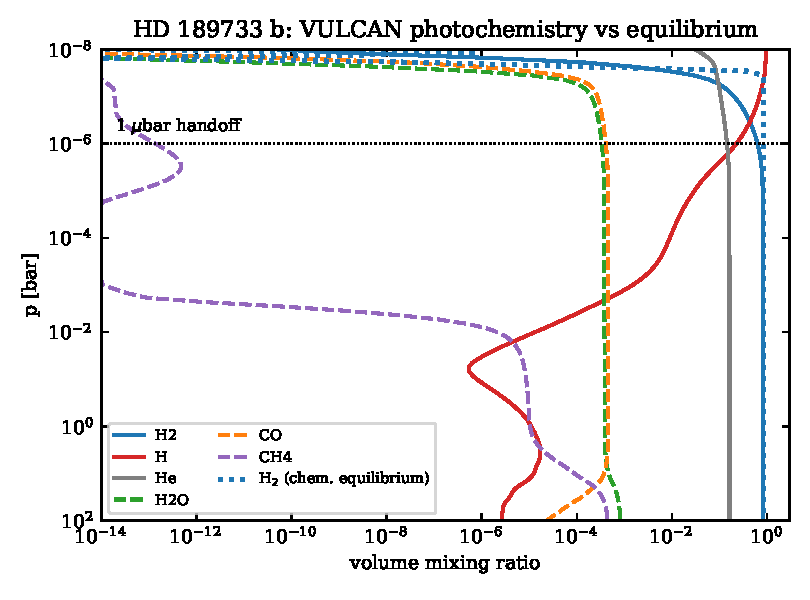
\includegraphics[width=0.62\textwidth]{fig_vulcan_vs_eq.pdf}
\caption{HD\,189733\,b lower/middle atmosphere from the converged VULCAN run
(solid/dashed: H$_2$, H, He, H$_2$O, CO, CH$_4$) compared with the
chemical-equilibrium H$_2$ mixing ratio evaluated along the same $T(p)$ (dotted).
Above $\sim$$10^{-4}$ bar photochemistry dissociates H$_2$ far beyond equilibrium; at
the 1\,$\ubar$ handoff (horizontal dotted line) $q_{\rm H}=0.23$ versus the
equilibrium 0.020: the $\sim$11$\times$ underestimate quantified.}
\label{fig:vulcan}
\end{figure}

% ===================================================================== %
\section{Example applications: HD and WASP planets}\label{sec:examples}
% ===================================================================== %

The approach was applied to the four planets modeled with EXHALE
(\texttt{examples/13\_lower\_atmosphere/}; $R_\mathrm{1bar}$ = broadband transit radius;
$T_\mathrm{eq}$, $M_\mathrm{p}$, He/H from each run's \texttt{input.inp}).

\begin{table}[h]\centering\small
\begin{tabular}{@{}lcccc cccc cc@{}}
\toprule
 & $M_\mathrm{p}$ & $T_\mathrm{eq}$ & He/H & $R_\mathrm{1bar}$ & input $R_0$ &
 \multicolumn{2}{c}{$r_0$(1\,$\ubar$) [$\RJ$]} & $r_0^\mathrm{Gui}$ & $\qHH$ & $\mu_\mathrm{base}$ \\
planet & [$M_\mathrm{J}$] & [K] & & [$\RJ$] & [$\RJ$] & chem.eq. & atomic & [$\RJ$] & (base) & [amu] \\
\midrule
HD\,209458\,b & 0.720 & 1450 & 0.0833 & 1.36  & 1.401  & 1.472 & 1.582 & 1.466 & 0.831 & 2.25 \\
HD\,189733\,b & 1.237 & 1183 & 0.0833 & 1.138 & 1.193  & 1.174 & 1.205 & 1.171 & 0.838 & 2.26 \\
WASP-121\,b   & 1.182 & 2358 & 0.0851 & 1.753 & 2.2075 & 2.010 & 2.133 & 1.966 & 0.005 & 1.24 \\
WASP-52\,b    & 0.460 & 1304 & 0.0204 & 1.27  & 1.270  & 1.437 & 1.615 & 1.428 & 0.837 & 1.95 \\
\bottomrule
\end{tabular}

\smallskip
\parbox{0.95\textwidth}{\footnotesize Isothermal-$T_\mathrm{eq}$ column (chem.\
equilibrium $+$ fully-atomic bracket) and the Guillot variant $r_0^\mathrm{Gui}$
($T_\mathrm{base}^\mathrm{Gui}$ = 1313, 1072, 2136, 1181\,K respectively).
``input $R_0$'' is the base radius currently used in the production runs.}
\end{table}

\begin{figure}[htb]\centering
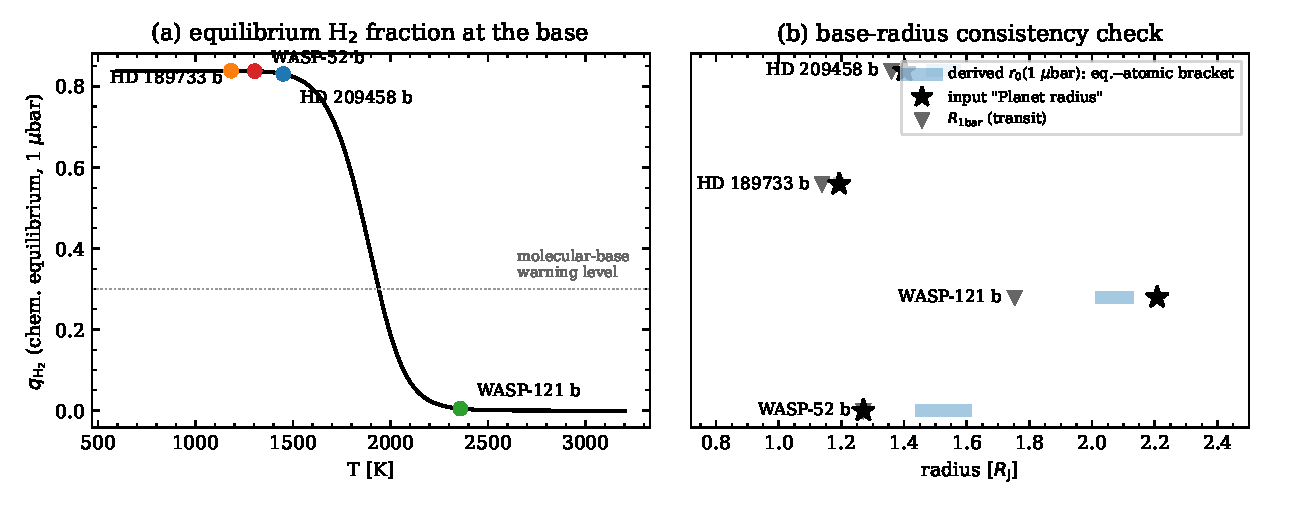
\includegraphics[width=\textwidth]{fig_lc_planets.pdf}
\caption{Tier-1 analytic column applied to the four planets. (a) The
chemical-equilibrium H$_2$ mixing ratio at 1\,$\ubar$ (Eq.~\ref{eq:visscher}) as a
function of temperature: the three $T_{\rm eq}\lesssim1500$\,K planets sit on the
fully molecular plateau, while WASP-121\,b ($T_{\rm eq}=2358$\,K) is atomic even in
equilibrium. (b) Derived 1-$\ubar$ base radius (equilibrium--atomic bracket, shaded)
versus the production ``Planet radius'' (star) and the transit radius (triangle):
HD\,189733\,b falls inside its bracket, HD\,209458\,b sits $\sim$5\% below,
WASP-121\,b lies just above (dayside-hot lower atmosphere), and WASP-52\,b's
transit-radius shortcut puts the base 0.17--0.35\,$\RJ$ too deep.}
\label{fig:lc}
\end{figure}

\noindent Interpretation (per planet):
\begin{itemize}
\item \textbf{HD\,189733\,b: consistent.} The production base radius (1.193\,$\RJ$)
  falls \emph{inside} the derived bracket [1.174, 1.205]: the adopted setup is validated
  by the column, not merely assumed.
\item \textbf{HD\,209458\,b: input $\sim$5\% low.} The production value 1.401\,$\RJ$
  sits just below the bracket [1.472, 1.582]. Given the isothermal-$T_\mathrm{eq}$
  assumption this is within the method's spread, but it suggests the 1-$\ubar$ level may
  lie slightly higher than assumed; the effect on $\Mdot$ is bounded by the Salz
  base-sensitivity results ($\lesssim10\%$-level).
\item \textbf{WASP-121\,b: the atomic base is \emph{verified}.} At
  $T_\mathrm{eq}=2358$\,K the equilibrium base is already atomic ($\qHH=0.005$,
  $q_\mathrm{H}=0.92$, $\mu=1.24$): for this ultra-hot Jupiter EXHALE's atomic assumption
  holds \emph{even in equilibrium}, with no appeal to photochemistry. The production base
  radius 2.2075\,$\RJ$ (derived earlier from the Huang et al.\ 2023 Table-3 $\log g$
  anchoring) lies $\sim$4--10\% above the isothermal-$T_\mathrm{eq}$ bracket [2.010,
  2.133]: consistent with a dayside lower atmosphere hotter than the
  redistribution-averaged $T_\mathrm{eq}$, which extends the column. Note the deep layers
  are still molecular ($\qHH(1\,\mathrm{bar})\approx0.83$), so $\mu$ varies from 2.25 to
  1.24 along this column: the equilibrium track is \emph{shorter} than the atomic
  bracket here because of its heavier deep-layer $\mu$.
\item \textbf{WASP-52\,b: misplaced base, impact quantified.} The production runs use
  the transit radius itself (1.27\,$\RJ$) as the 1-$\ubar$ base, the common shortcut,
  but the column places that level at 1.44--1.62\,$\RJ$, i.e.\ the base is
  0.17--0.35\,$\RJ$ (13--27\%) too deep. \emph{Recomputation} (the
  \texttt{fxuv1p0\_he98} configuration rerun Newton-converged with the corrected
  equilibrium-column base $r_0=1.437\,\RJ$, all else identical): $\log\Mdot$
  $11.97\to12.14$ ($\times1.5$), but the He\,10830 observable barely moves,
  line-center absorption $27.11\to27.56\%$ ($\times1.02$) and equivalent width
  $0.713\to0.722$\,\AA\ ($\times1.01$). The line-forming effective radius is set by
  the $\tau{=}1$ surface of the extended wind, which stays nearly fixed in
  \emph{physical} units (the larger, less-bound base raises $\Mdot$, but the He\,2$^3$S
  column at a given physical radius is almost unchanged: peak $n_{\mathrm{2^3S}}$
  150.5$\to$147.6\,cm$^{-3}$). Conclusion: the base misplacement biases the
  \emph{mass-loss rate} at the $\times1.5$ level but appears not to bias the He\,10830
  scan conclusions materially. Figure~\ref{fig:w52} shows the two line profiles. Also note this run family's low He/H ($=0.0204$, the
  ``He98'' abundance scan), visible in the light $\mu_\mathrm{base}$.
\item \textbf{Common pattern.} All three $T_\mathrm{eq}\lesssim1500$\,K planets have
  strongly molecular \emph{equilibrium} bases ($\qHH\approx0.83$, the fully-molecular
  limit of the fit): quantifying that their atomic bases rest on \emph{photochemical}
  dissociation (Moses et al.\ 2011; Koskinen et al.\ 2013a) rather than thermal, which is
  precisely what the Tier-3 \texttt{VULCAN} upgrade would supply from first principles.
  The Guillot column is systematically slightly more compact (cooler skin above the
  photosphere): a $\lesssim$0.5\% radius effect at fixed assumptions.
\end{itemize}

\begin{figure}[htb]\centering
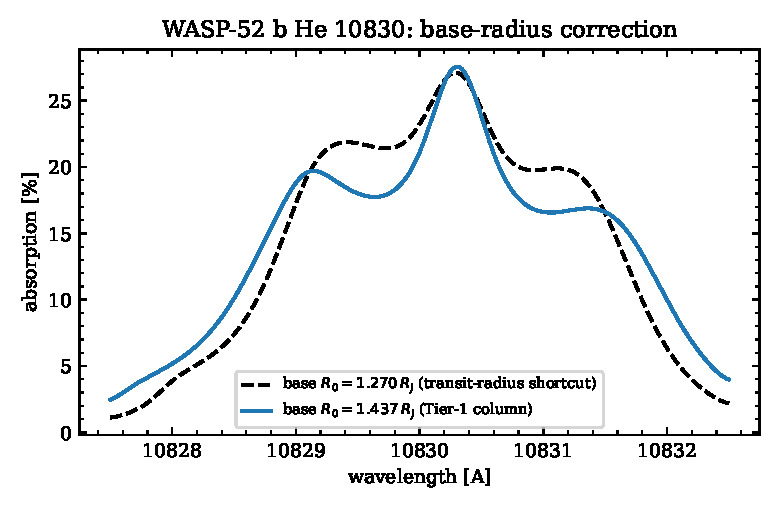
\includegraphics[width=0.6\textwidth]{fig_w52_he10830.pdf}
\caption{WASP-52\,b He\,10830 transmission (instrument$+$rotation convolved) for the
old transit-radius-shortcut base ($R_0=1.270\,\RJ$, dashed) and the corrected Tier-1
column base ($R_0=1.437\,\RJ$, solid), both Newton-converged with the same binary. The
line core (27.11 vs.\ 27.55\%) and equivalent width (0.713 vs.\ 0.722\,\AA) are
essentially unchanged (the $\tau{=}1$ line-forming surface of the extended wind is
fixed in physical units) with only a mild reshaping of the shoulders; the base
misplacement instead biases $\Mdot$ ($\log\Mdot$ 11.97$\to$12.14, $\times$1.5).}
\label{fig:w52}
\end{figure}

% ===================================================================== %
\section{Using and connecting the results}\label{sec:usage}
% ===================================================================== %

\subsection{Recommended workflow for each planet}
\begin{enumerate}
\item \textbf{Column check (always, free).} Add \texttt{Lower column: <transit radius>}
  to \texttt{input.inp} (or run \texttt{run\_lower.py}). Read off: does the current
  ``Planet radius'' fall inside the [chem.eq., atomic] bracket? Is $\qHH$(base) small?
\item \textbf{Decide the tier.} $\qHH\lesssim0.1$ (e.g.\ WASP-121\,b): the atomic model
  is verified, proceed as usual. $\qHH\sim0.8$ with $T_\mathrm{eq}\sim1000$--2000\,K
  (typical hot Jupiters): the atomic base rests on photochemistry, proceed, but note
  the assumption; a genuinely cool planet (warm Neptune / sub-Neptune) needs Tier-2
  physics before its He\,10830 predictions are trusted.
\item \textbf{Adopt the geometry.} If the input radius lies outside the bracket
  (WASP-52\,b), either correct ``Planet radius'' by hand or copy the driver's
  \texttt{base.inp} into the run directory so EXHALE adopts $r_0$, $T_0$, He/H and
  $K_{zz}$ automatically (echoed at startup).
\item \textbf{Run EXHALE} with the usual two-stage convergence ($+$ Newton finish for
  quantitative $\Mdot$), then \texttt{EXHALE\_}\allowbreak\texttt{transit.py} for
  the transit spectra.
\item \textbf{(Optional) iterate} once a real lower-atmosphere model is attached
  (\S\ref{sub:feedback}).
\end{enumerate}

\subsection{Where each quantity connects}
\begin{center}\small
\begin{tabular}{@{}p{3.6cm}p{2.9cm}p{9.2cm}@{}}
\toprule
quantity & produced by & consumed by / effect \\
\midrule
$r_0$(1\,$\ubar$) & Tier 1 / \texttt{base.inp} & grid inner radius, gravity $b_0$,
  irradiated area; TPM continuum radius \\
bracket $[r_0^\mathrm{eq}, r_0^\mathrm{atom}]$ & Tier 1 & consistency check on the input
  radius; systematic-error bar on $r_0$ \\
$T_\mathrm{base}$ & driver ($T_\mathrm{eq}$ or Guillot) & thermal BC $T_0$; $v_0$, $p_0$,
  $b_0$ normalization \\
$\qHH$(base) & Eq.~\eqref{eq:visscher} & tier-decision switch; \texttt{Molecular base}
  correction; Tier-2 initial condition \\
He/H (base) & \texttt{base.inp} & composition; the \texttt{He\_diffusion} reservoir value \\
$K_{zz}$ & \texttt{base.inp} & \texttt{he\_kzz}: homopause of the He/H (and metal)
  diffusive separation \\
$\Lambda_{\mathrm{H_3^+}}(T,n_{\mathrm{H_3^+}},n_\mathrm{H_2})$ & \texttt{h3p\_cooling} &
  (Tier 2) new term in the \texttt{cool} array of the energy equation \\
R1--R23 rates & \texttt{mol\_rates} & (Tier 2) source terms of
  \texttt{System\_HeH\_mol}; H$_3^+$/HeH$^+$ densities for the cooling and for
  IR-diagnostic post-processing \\
metal release $n_X/n_\mathrm{H}$ & (Tier 3, VULCAN) & \texttt{metals.inp} values,
  replaces assumed solar totals for the Mg\,II/Ca\,II/Na\,I transmission lines \\
\bottomrule
\end{tabular}
\end{center}

\subsection{Feedback loop}\label{sub:feedback}
One-way coupling (lower $\to$ \texttt{base.inp} $\to$ EXHALE, with the Taylor-style
tolerated composition discontinuity) is the default.

\paragraph{The elemental-flux closure is implemented (2026-08-27).} The two-way
iteration runs on the elemental fluxes, driven by
\texttt{src/utils/element\_flux\_closure.py}. The chemistry is told a trial
elemental flux through its upper boundary
(\texttt{-{}-trial-flux-H}/\texttt{-{}-trial-flux-He} of
\texttt{photochem\_to\_lower\_profile.py}, g\,s$^{-1}$ outward positive: the
Lavvas et al.\ 2014 prescription in flux form), the resulting profile becomes the
wind's base state, and the wind's own elemental flux is measured face by face by
\texttt{write\_element\_flux\_profile} (\texttt{binary\_element\_diffusion.f90}),
\[
  F_{\rm He}=4\pi r^2(\rho X v + J),\qquad
  F_{\rm H}=4\pi r^2(\rho(1-X)v - J),
\]
and reduced to one median and one relative spread per element over a radial
window. The solution is the fixed point $\Phi_{\rm El}=F_{\rm El}(\Phi_{\rm El})$,
reached by an under-relaxed update $\Phi^{(k+1)}=\Phi^{(k)}+\omega(F^{(k)}-\Phi^{(k)})$
with $\omega=0.5$ halved (floor $0.125$) whenever the residual fails to fall. The
convergence test reads the \emph{undamped} residual, so a small $\omega$ cannot
buy a false convergence, and a residual smaller than the spread of the window it
was measured on is reported \texttt{UNRESOLVED} rather than converged. The driver
reads the overlap window first and falls back on the steady window $r\ge r_{\rm esc}$
when the overlap is unmeasurable or too ragged, recording which window supplied
the number. Design: \texttt{docs/phase\_e\_flux\_closure\_design.md} \S6.

\paragraph{Still one-way.} The radiation half of the loop is not implemented.
EXHALE already computes the attenuated stellar spectrum on its energy grid, so the
\emph{transmitted XUV flux at the base}, $F_\nu(r_0)=F_\nu e^{-\tau_\nu(r_0)}$, could be
dumped and handed to the photochemical model as its top irradiation; today the
adapters take a stellar flux file and a dilution instead. Taylor et al.\ found
$\sim$3 iterations sufficient for the analogous Ly$\alpha$ loop; the same is
expected here since the wind is insensitive to base details at the $\lesssim$10\%
level (Salz et al.\ 2016).

\subsection{The element operator: what it conserves, and where its
boundary comes from}
\label{sub:elemop}

The closure above rests on the same operator that carries the He/H and metal
separation through the wind, \texttt{binary\_element\_diffusion.f90}. Three
statements about it were settled on 2026-09-10 and belong beside the flux
numbers, because two of them change what those numbers mean.

\paragraph{The projection now conserves the mixture mass.} After each
element update the species vector is projected back onto the new element
totals by \texttt{project\_elements}. It used to take the mixture mass as
$m_{\rm sum} = m_1 n_{\rm H} + m_{\rm He} n_{\rm He}$ with $m_1$ the
\emph{reservoir} mass per hydrogen nucleus, i.e.\ the trace metals at their
\texttt{metals.inp} abundances, while the cell carries its metals at whatever
the trace transport left it. The difference was written into hydrogen at
every call. MEASURED at one cell of the certification column whose metal/H
was $0.024401$ against the reservoir's $0.028227$, $\sum_i m_i f_i$ went
$1.0000000 \rightarrow 1.0000636$ in a single step: mass created. A second
leak of the same kind: the trace-metal transport wrote metal densities with no
counter-flux in the hydrogen they diffuse through
($3.0\times10^{-3}$ on the suite column with the metals frozen).

\texttt{mixture\_mass\_split} now reads the mass the cell's species actually
carry, component~1 is scaled as a whole, and one projection after the metal
loop puts the metals' mass change back onto hydrogen. Mass closure of the
certification column after the relaxation went $3.37\times10^{-3} \rightarrow
2.3\times10^{-15}$, and of the handed-back atomic candidate $6.44\times
10^{-3} \rightarrow 1.94\times10^{-9}$, the file's own precision. A run with
metals off is unaffected by construction ($m_1 = m_{\rm H} = 1$ exactly).
The counter-flux is closed on hydrogen but not on momentum or internal
energy; that is a trace approximation and is named as one at the routine.

This is not a cosmetic repair for anyone using the coupling: the
\texttt{lower\_profile} regression case, the one that hands the lower
atmosphere over as a profile, had a stored reference $3.6\times10^{-4}$ out
of closure (O/H $4.61\times10^{-4}$ against the reservoir's
$4.90\times10^{-4}$). A $1500$-step cold start goes $6.77\times10^{-3}
\rightarrow 3.14\times10^{-9}$ in closure, with $T$ at $1.6\,R_{\rm p}$
moving $1.3\%$ and H\,\textsc{i} $6.3\%$. Its reference was re-snapshotted at
the 2026-09-10 gate.

\paragraph{The boundary of the residual is the caller's, deliberately.} The
two relaxation solvers (\texttt{element\_diffusion\_step},
\texttt{solve\_trace\_element\_in\_hydrogen}) refill the upper ghosts of
their own working arrays before every pass, while
\texttt{element\_transport\_residual}, which measures the same balance on a
state, reads the ghosts the caller left. Making the residual pose its own
zero-gradient top was tried and reverted. It is physically the right
condition and it changes the residual by one element's outermost row in its
twelfth digit and nothing else (the production callers already hand the
operator ghosts equal to the cell to one to four units in the last place),
but the atomic element rows of the stationary solve do not survive a
last-bit change of those ghosts, whatever makes it: a control that merely
multiplies the same three ghost quantities by $1 + 2\times10^{-16}$ and poses
no boundary at all moves them just as far. The amplifier is the Krylov leg
at its one-digit tolerance, which crosses that tolerance on a different
vector and sends the acceptance test down a different branch a few
iterations later. The asymmetry therefore stays in the tree, documented at
the routine and measured by \texttt{src/tests/element\_operator/}, which
asserts the size of the caller dependence ($1.19\times10^{-2}$ of the row's
scale on a stale caller) rather than assuming it away.

\paragraph{The open item: the layer does not conserve the element flux.} The
window reduction of the flux closure above is also the honest statement of
how well the operator conserves what it transports. MEASURED on the atomic
candidate state, as the relative radial spread of $F_{\rm El}$ about its
median:

\begin{center}\small
\begin{tabular}{@{}lccc@{}}
\toprule
window & $F_{\rm He}$ spread & $F_{\rm H}$ spread & face mass-flux spread \\
\midrule
layer, $r < 1.10$        & $9.79$               & $9.09$               & $9.25$ \\
wind, $r \ge 1.20$       & $2.71\times10^{-2}$  & $1.36\times10^{-2}$  & $3.99\times10^{-3}$ \\
escape, $r \ge 2.0$      & $2.01\times10^{-3}$  & $2.14\times10^{-3}$  & $1.55\times10^{-3}$ \\
\bottomrule
\end{tabular}
\end{center}

\noindent The mass-flux spread the same state is usually quoted with,
$9.8\times10^{-7}$, is a \emph{cell-centered} number and says nothing about
these: the element fluxes are three to four decades worse in the same state.
The projection fix buys a factor four in the layer ($39.3 \rightarrow 9.79$
for helium) and nothing in the wind, which is what a mass-closure repair
should do, since the leak was largest where the composition changes most. A
spread of $9.8$ means the layer's element fluxes are not conserved at all,
and the standing base wave is the suspect. The consequence has been taken:
the certification gates the element and carrier rows only at $r \ge 1.20$,
and the layer's rows are reported and do not gate until this number is
repaired; \texttt{certification.f90} states that reason at the declaration of
its two regime radii. Numbers here are READ from
\texttt{docs/certification\_tolerance\_anchoring\_20260910.md} section~5.

\subsection{Consistency cautions}
\begin{itemize}
\item Do not double-count composition: if \texttt{base.inp} sets He/H from a lower model,
  the \texttt{metals.inp} abundances should be the same model's \emph{atomic release}
  values, not solar totals.
\item \texttt{base.inp} overrides win over \texttt{input.inp} for $T_0$, $R_0$, He/H
  (echoed); remove the file to return to the manual values.
\item The Tier-1 column is isothermal and spherical: near-RLO planets (WASP-121\,b) need
  the Roche correction before the bracket is taken quantitatively, and dayside-hot lower
  atmospheres extend beyond the $T_\mathrm{eq}$ column (both visible in the WASP-121\,b
  example above).
\item The \texttt{Molecular base} key changes only the EOS budget; do not combine it with
  quantitative He\,10830 claims for genuinely cool planets: that is Tier-2 physics.
\end{itemize}

% ===================================================================== %
\section{Converged Tier-2 solutions (2026-08-13)}\label{sec:converged}
% ===================================================================== %

Every Tier-2 number quoted above comes from a 12000-step relaxation snapshot:
until 2026-08-13 no molecular configuration in the tree had ever reached a steady
state (\texttt{examples/15\_molecular} ran 135694 steps to $du=2.9\times10^{-2}$).
The first Newton-converged molecular solutions were obtained on the hot-Uranus
gate (\texttt{lower\_atmosphere\_figs/data\_g2/input.inp}, the configuration the
\texttt{mol\_base\_handoff} regression case runs, $\qHH^\mathrm{base}=0.75$) once
the H$_3^+$ infrared cooling was moved inside \texttt{eval\_cool}
(\texttt{docs/Update\_EXHALE.pdf} \S54), so that the marching temperature update
and the steady residual balance the same cooling function.

\paragraph{Recipe.} Three keys, and they are the whole change:
\begin{center}
\texttt{Solver: Newton 5.0e-2} \quad
\texttt{Resid tol: 1.0e-5} \quad
\texttt{Max steps: 150000}
\end{center}
\texttt{Solver: Newton 5.0e-2} raises the hand-off threshold, because the $du$
descent of a molecular run is \emph{not monotonic} (on the hot-Uranus gate it
reaches $8.8\times10^{-2}$ near step 11500 and bounces back to $7\times10^{-1}$
before resuming), so a run can spend its whole step budget above the
$10^{-2}$ default. \texttt{Max steps: 150000} covers the marching warm-up.
Marching alone can \emph{never} reach the molecular layer: its H$_3^+$ cooling
time is $1.3\times10^{7}$\,s at $r=1.02$ against a CFL-limited step of 0.30\,s,
i.e.\ $4\times10^{7}$ steps per cooling time. It is the Newton solve that
reaches it.

\paragraph{The default residual target is too loose for a molecular run.}
$\|R\|$ is the maximum relative residual over the wind, and in a molecular run it
is set by the first two or three cells above the base, where the energy residual
is ${\sim}10^{3}$ times the value anywhere else. Stopping at the default
$\|R\|<10^{-3}$ therefore leaves the molecular layer still cooling: its
cell-by-cell energy residual is then 0.7$\times$ the local H$_3^+$ cooling rate,
with the same sign in 173 of 180 cells. Re-solving the same state with
\texttt{Resid tol: 1.0e-5} moves the layer again (by 60--70\% in $T$), and
only there does the solution become a fixed point of the procedure: a third solve
reproduces $T$ to $\le0.14\%$ and the H$_2\to$H front to five digits.
\textbf{A molecular run needs \texttt{Resid tol: 1.0e-5}.}

\begin{center}\small
\begin{tabular}{@{}lcc@{}}
\toprule
hot-Uranus gate & metals off & metals on (solar C/N/O/Mg/Ca/Na/Fe) \\
 & snapshot $\to$ converged & snapshot $\to$ converged \\
\midrule
residual norm at exit & $6.7\times10^{-7}$ & $1.4\times10^{-6}$ \\
H$_2\to$H front ($x_{\rm H_2}=0.5$) & $1.16037\to\mathbf{1.03581}$ & $1.16244\to\mathbf{1.07974}$ \\
base $T$ (cell 1, pinned by the BC) & $1213.42\to1212.86$\,K & $1213.46\to1213.45$\,K \\
H$_3^+$ peak [cm$^{-3}$] & $7.03\!\times\!10^{4}$@1.0419 $\to$ $\mathbf{3.75\!\times\!10^{5}}$@1.0148 & $52.1$@1.1355 $\to$ $\mathbf{1.01\!\times\!10^{3}}$@1.0789 \\
$T$ at $r=1.02$ & $1304.9\to\mathbf{299.0}$\,K & $1312.8\to\mathbf{928.5}$\,K \\
$T$ at $r=1.08$ & $1302.6\to1075.5$\,K & $1319.8\to\mathbf{208.9}$\,K \\
$\log_{10}\Mdot$ [g/s], spherical & (not flat) $\to$ 10.542 & (not flat) $\to$ 10.599 \\
mass-flux spread, $r>1.2$ & $2.3\!\times\!10^{2}$--$3.8\!\times\!10^{3}\to2.4\times10^{-3}$ & idem \\
\bottomrule
\end{tabular}
\end{center}

\noindent The snapshot $\Mdot$ is quoted only because the code prints it: its mass
flux varies by a factor $2\times10^{2}$--$4\times10^{3}$ across the wind, so no
single number represents it.

\paragraph{What the converged solution says physically.} The molecular layer
collapses to 190--300\,K (far below $T_\mathrm{eq}=1140$\,K), and stops there
because the coolant switches itself off: the H$_3^+$ cooling time at $r=1.02$
rises from $1.3\times10^{7}$\,s in the snapshot to $1.3\times10^{10}$\,s in the
converged state. With metals the collapse is instead accompanied by the saturated
ground-term fine-structure lines (C\,I 609/370\,$\mu$m at the base, [O\,I]
63/145\,$\mu$m above it: 89\% and 91\% of the local cooling at $r=1.002$ and
1.040), and H$_3^+$ never exceeds 2.3\%. Either way the layer is cooled by lines
treated as \emph{optically thin}, with no thermal-infrared heating from below and
no radiative equilibrium: the base temperature is pinned in one cell by the
boundary condition and nothing holds the column above it. A real H$_2$ atmosphere
at these column densities is optically thick in exactly these lines and sits near
the radiative--convective profile. The converged Tier-2 thermal structure should
therefore be read as \textbf{the steady state of the model as written, and as a
quantitative statement that the model was missing an infrared escape probability
below the H$_2\to$H front}, not as a prediction of the temperature of a warm
Neptune's lower thermosphere. \S\ref{sec:baseir} supplies part of what is missing
and measures how far it goes. The wind above the front is much less affected:
$\Mdot$ moves 0.085\,dex (metals off) and 0.043\,dex (metals on) between the
$10^{-3}$ and $10^{-5}$ solutions, because it is launched above the collapsed
layer.

\paragraph{HD\,209458\,b: the same recipe on a real planet.} The second
Newton-grade molecular solution is \texttt{examples/}\allowbreak\texttt{15\_molecular}: the
metals-off HD\,209458\,b configuration of Gate 1, the one that had run 135694
steps without ever converging. The three keys above are the whole change: no warm
restart was needed, the run went from the default cold IC to \texttt{info = 0} in
one pass, 10\,min 25\,s on 8 threads. PLM\,$\to$\,WENO3 at step 13299, secondary
ionization flipped in at step 23837, JFNK engaged at step 25837 and took $\|R\|$
from $4.031\times10^{-2}$ to $\mathbf{9.542\times10^{-6}}$ in 272 iterations. Here
too the $du$ descent is not monotonic. The residual is dominated by the same
place: the worst cell is $j=1$--3, $r\approx1.000$--1.001, for 267 of the 272
iterations, split about evenly between the momentum and the energy row.

\begin{center}\small
\begin{tabular}{@{}lcc@{}}
\toprule
HD\,209458\,b, metals off & 12000-step snapshot & converged ($\|R\|=9.5\times10^{-6}$) \\
\midrule
H$_2\to$H front ($x_{\rm H_2}=0.5$) & 1.01975 & \textbf{1.00891} \\
base $T$ (cell 1, pinned by the BC) & 1466.55\,K & 1466.36\,K \\
$T$ at $r=1.005/1.02/1.08$ & 1909 / 1916 / 2855\,K & \textbf{401} / 2206 / 7574\,K \\
coldest cell below $r=1.3$ & 1463.6\,K @ 1.0002 & \textbf{397.3\,K @ 1.0056} \\
H$_3^+$ peak & $9.57\times10^{4}$\,cm$^{-3}$ @ 1.0004 & $\mathbf{5.18\times10^{5}}$\,cm$^{-3}$ @ 1.0017 \\
$x_{\rm H_2}$ at the base & 0.9964 & 0.9963 \\
$\log_{10}\Mdot$ [g/s], spherical & 10.873 & 10.532 \\
mass-flux spread over $r>1.05$ & 1.23 & $\mathbf{4.2\times10^{-3}}$ \\
\bottomrule
\end{tabular}
\end{center}

\noindent The solution is a fixed point of the procedure: re-solving from it with
the same tolerance returns \texttt{info = 0} at $\|R\|=9.0\times10^{-6}$ and
reproduces the front to 1.00879 (0.01\%), $\Mdot$ to 0.002\,dex and the H$_3^+$
peak to 0.4\%; only the coldest cell of the collapsed layer still moves
(397\,$\to$\,353\,K). Note the reload does not preserve the residual:
\texttt{Load IC? True} re-derives the ionization state from the file, so the
second solve starts at $\|R\|=8.7\times10^{-4}$. The physical reading is the
hot-Uranus reading, on a hot Jupiter: the molecular layer between the base and the
front collapses to ${\sim}400$\,K, H$_3^+$ carries \textbf{100\%} of the radiative
cooling from the base out to $r\approx1.005$ ($10^{4}$ times the local
photoheating at the base), and the same optically thin treatment applies. The
front moves inward by 0.011\,$\Rp$ and $\Mdot$ falls by 0.34\,dex relative to the
snapshot, so for HD\,209458\,b the relaxation-snapshot $\Mdot$ is \emph{not} a
substitute for the converged one.

\paragraph{With metals the same planet does not converge.}
\texttt{examples/16\_molecular\_metals} (the identical configuration plus solar
C/N/O) under the same three keys reaches the hand-off
(PLM\,$\to$\,WENO3 at step 15263, secondary ionization at 61158), and the JFNK
then stalls: $\|R\|$ falls from $2.338\times10^{-2}$ to $3.6\times10^{-4}$ over
281 iterations and the line search finds no descent step for 12 consecutive
iterations (\texttt{info = 2}, worst cell $j=93$, $r=1.021$, momentum), after
which the run reverts to marching. This is the reverse of the hot-Uranus gate,
where the metals-on case converged as readily as the metals-off one, and it is the
base-adjacent momentum stall recorded as item (A) of \texttt{TO\_BE\_DONE.md},
displaced outward to the front. \texttt{16\_molecular\_metals} therefore carries
the plain \texttt{Solver: Newton} line and has no converged solution.

% ===================================================================== %
\section{The infrared field of the lower atmosphere
(\texttt{Base IR field})}\label{sec:baseir}
% ===================================================================== %

The converged Tier-2 solutions above left one question open: why does the
molecular layer sit at 190--300\,K, and is the optically thin line cooling the
cause? The measurement below says the suspect is the right one for the metals-off
case and the \emph{wrong} one for the metals-on case, and the closure follows the
measurement.

\paragraph{What the lines actually see.} Line-center optical depths of the eight
ground-term fine-structure lines, from the converged metals-on solution of the
hot-Uranus gate, with the level populations and Doppler widths the cooling module
itself uses. $\tau_\mathrm{up}$ is the column from the cell to the top of the
domain (the one the escape probability was built from), $\tau_\mathrm{dn}$ the
column to the bottom.

\begin{center}\small
\begin{tabular}{@{}cccccccc@{}}
\toprule
$r/\Rp$ & $T$ [K] & $\tau_\mathrm{up}$(C\,I 609) & $\tau_\mathrm{dn}$ & $\beta$
 & $\tau_\mathrm{up}$([O\,I] 63) & $\tau_\mathrm{dn}$ & $\beta$ \\
\midrule
0.9998 & 1213 & 0.088 & $1.7\times10^{-4}$ & 0.904 & 2.01  & $4.0\times10^{-3}$ & 0.211 \\
1.0102 & 1033 & 0.069 & 0.019 & 0.924 & 1.57  & 0.44 & 0.265 \\
1.0302 &  820 & 0.040 & 0.048 & 0.955 & 0.89  & 1.1  & 0.421 \\
1.0501 &  573 & 0.020 & 0.068 & 0.978 & 0.43  & 1.6  & 0.633 \\
1.0749 &  289 & 0.005 & 0.083 & 0.995 & 0.093 & 1.9  & 0.898 \\
1.0832 &  188 & 0.001 & 0.086 & 0.998 & 0.028 & 2.0  & 0.968 \\
\bottomrule
\end{tabular}
\end{center}

\noindent So \textbf{escape was never the problem}: outward the collapsed layer is
thin ($\beta\ge0.90$ for C\,I, $\ge0.63$ for [O\,I] above $r=1.05$), and trapping
can only reduce the cooling by a factor of a few at the base. What the treatment
left out is the \emph{other} direction. The gas below the base is not vacuum.
Taking the base cell opacity and one pressure scale height of an isothermal
exponential reservoir (base pressure 9.0\,$\ubar$):

\begin{center}\small
\begin{tabular}{@{}lccc@{}}
\toprule
line & $\tau$ per scale height at the base & pressure where $\tau=1$ & $\tau$ at 1 bar \\
\midrule
{}[O\,I] 63\,$\mu$m  & 1.08  & 17\,$\ubar$  & $1.2\times10^{5}$ \\
{}[O\,I] 145\,$\mu$m & 0.32  & 37\,$\ubar$  & $3.6\times10^{4}$ \\
C\,I 370\,$\mu$m     & 0.092 & 106\,$\ubar$ & $1.0\times10^{4}$ \\
C\,I 609\,$\mu$m     & 0.046 & 205\,$\ubar$ & $5.1\times10^{3}$ \\
C\,II 158, N\,II 205/122, [O\,I] 44\,$\mu$m & $\le1.2\times10^{-10}$ & - & $\le3\times10^{-2}$ \\
\bottomrule
\end{tabular}
\end{center}

\noindent Every line that carries the cooling is black downward within one to
three scale heights below the model base. The layer therefore faces a blackbody,
not a void, and the ratio of the incident mean intensity to the line source
function, $\bar J/S = \tfrac12 B_\nu(T_\mathrm{base})/B_\nu(T)$, crosses 1
wherever $T$ drops below ${\sim}610$\,K: at the coldest cell it is 3.4 (C\,I
609\,$\mu$m) to 5.7 ([O\,I] 63\,$\mu$m). Those lines were being made to cool a gas
that they should have been heating.

\paragraph{But that is not what makes the metals-on layer cold.} Two measurements
say the fine-structure lines are not the cause of the 190--300\,K there.
\begin{itemize}
\item \textbf{The specific entropy rises monotonically outward through the whole
  collapsed layer}, $p/\rho^{\gamma}$ going from 1.00 at the base to 1.67 at
  $r=1.05$ and 5.69 at $r=1.083$. The gas is net heated everywhere; it is cold
  because $\rho$ has fallen by a factor $10^{2}$. The layer is an expansion, not a
  radiative collapse.
\item \textbf{The metals-off solution collapses further with no fine-structure
  cooling at all}: 115\,K at $r=1.033$, where its total cooling is
  $3.8\times10^{-12}$\,erg\,cm$^{-3}$\,s$^{-1}$.
\end{itemize}
The energy budget makes the same point directly: the metals-on cooling is 36\% of
the local photoheating at $r=1.01$ and 2--16\% above $r=1.02$, and
$\mathrm{heat}-\mathrm{cool}$ is balanced by the expansion term
$\rho v[\mathrm{d}\varepsilon/\mathrm{d}r + p\,\mathrm{d}(1/\rho)/\mathrm{d}r]$ to
within a few percent. The one place radiation dominates is the metals-off base:
there H$_3^+$ carries 100\% of the cooling, the entropy \emph{falls} by a factor 3
between the base and $r=1.02$, and the layer really is radiating itself down.

\paragraph{The closure.} \texttt{Base IR field: True} (default \texttt{False})
gives both families of infrared coolant the field they sit in. The lower
atmosphere is taken to be black at their wavelengths and to radiate $B_\nu(T_0)$
over the sky fraction $f = 1-\sqrt{1-(\Rp/r)^{2}}$, i.e.\ the whole lower
hemisphere at the base and the usual dilution far away.

For the eight fine-structure lines the incident field enters \emph{inside} the
ground-term statistical equilibrium, as the photon occupation number
\begin{equation}
  \bar n \;=\; \frac{\beta_1(\tau_\mathrm{dn})\,f}{\exp(E_{ul}/kT_0)-1},
\end{equation}
with radiative rates $\beta A(1+\bar n)$ down and $\beta A (g_u/g_l)\bar n$ up, so
the returned power is the \emph{net} one, emission minus absorption. The escape
probability becomes two-sided, $\beta=\beta_1(\tau_\mathrm{up})+
\beta_1(\tau_\mathrm{dn})$ with $\beta_1$ the single-face Hollenbach \& McKee
(1979) / de Jong et al.\ (1980) form; with the field off it reduces to
$2\beta_1(\tau_\mathrm{up})$, the previous value, bit for bit. Each line then
stops cooling at its own radiative equilibrium temperature, 575.8\,K (C\,I
609\,$\mu$m) to 641.7\,K ([O\,I] 44\,$\mu$m) for $T_0=1140$\,K and half-sky
coverage, and heats below it.

For H$_3^+$ there is no line list (Miller et al.\ (2013) fit the \emph{total}
emission), so the absorption is taken from that fit at the radiating
temperature, which is what Kirchhoff's law makes of an emission integral:
$\Lambda_\mathrm{net}=n(\mathrm{H_3^+})\,4\pi\,s(T,n_{\mathrm{H_2}})
\,[E(T)-W\,E(T_0)]$. This is the same net-exchange form the H$_2$, H$_2$O and CO
channels use (\S\ref{sec:molir}), and it is bounded at every temperature. Its
radiative equilibrium temperature is 975.4\,K at the base for $T_0=1140$\,K.
Between 2026-08-13 and 2026-08-31 the exchange was instead closed on one
effective band, the $\nu_2$ fundamental at 2521.3\,cm$^{-1}$ ($E/k=3627.5$\,K),
as $\Lambda_\mathrm{net}=\Lambda_\mathrm{emit}(T)\,[1+\bar n-\bar n\,e^{E/kT}]$,
with equilibrium temperatures of 936.1\,K and then 941.2\,K. Pairing a total
emission fit with the Boltzmann factor of one of its transitions diverges below
about 150\,K and is wrong by a factor 1.5--1.9 over 400--1000\,K; \S112 of
\texttt{docs/Update\_EXHALE.pdf} measures it and records what moved.
The approximations and where they break are written at
\texttt{h3p\_net\_cooling\_rate}
(\texttt{src/modules/lower\_atmosphere/h3p\_cooling.f90}) and at
\texttt{fine\_structure\_line\_transfer}
(\texttt{src/modules/radiation/Cool\_coeff.f90}). Fe\,II (a precomputed
statistical-equilibrium table), the coronal remainders and every permitted line
keep the optically thin, no-incident-field limit; the estimated heating the
remainders would add is ${\sim}0.4\%$ of the losses of this layer.

\paragraph{What it does.} Both runs restart the converged
\texttt{Resid tol: 1.0e-5} solutions of \S\ref{sec:converged} with the switch on,
and both return \texttt{info = 0}.

\begin{center}\small
\begin{tabular}{@{}lcccc@{}}
\toprule
hot-Uranus gate & \multicolumn{2}{c}{metals off} & \multicolumn{2}{c}{metals on} \\
\cmidrule(lr){2-3}\cmidrule(lr){4-5}
 & field off & \textbf{field on} & field off & \textbf{field on} \\
\midrule
residual norm at exit & $6.7\!\times\!10^{-7}$ & $1.3\!\times\!10^{-6}$ & $1.4\!\times\!10^{-6}$ & $9.9\!\times\!10^{-6}$ \\
$T$ at $r=1.005$ & 626.8\,K & \textbf{910.0\,K} & 1099.0\,K & 1098.9\,K \\
$T$ at $r=1.02$  & 299.6\,K & \textbf{859.4\,K} &  928.9\,K &  928.9\,K \\
$T$ at $r=1.03$  & 140.2\,K & \textbf{840.2\,K} &  820.0\,K &  820.1\,K \\
$T$ at $r=1.05$  & 476.8\,K & \textbf{753.0\,K} &  573.0\,K &  573.4\,K \\
coldest cell & 115.1\,K @ 1.0334 & \textbf{229.7\,K @ 1.0947} & 187.9\,K @ 1.0831 & 189.1\,K @ 1.0831 \\
H$_2\to$H front & 1.03582 & \textbf{1.08833} & 1.07976 & 1.07979 \\
H$_3^+$ peak [cm$^{-3}$] & $3.75\!\times\!10^{5}$ & $3.19\!\times\!10^{5}$ & $1.01\!\times\!10^{3}$ & $1.00\!\times\!10^{3}$ \\
$\log_{10}\Mdot$, spherical & 10.539 & 10.617 & 10.596 & 10.596 \\
mass-flux spread, $r>1.2$ & $2.4\!\times\!10^{-3}$ & $2.4\!\times\!10^{-3}$ & $2.4\!\times\!10^{-3}$ & $2.4\!\times\!10^{-3}$ \\
\bottomrule
\end{tabular}
\end{center}

\noindent\textbf{Stale, and not re-measurable from here: the field-on columns
and the predicted floors below were computed with the single-band H$_3^+$
closure, which was replaced on 2026-08-31 (\S112 of
\texttt{docs/Update\_EXHALE.pdf}).} The converged solutions they restart from no
longer exist as run directories, so the table is left as the record of what that
closure gave. The same four-way comparison re-measured with the current closure,
at the 12000-step protocol of the \texttt{mol\_ir\_bands} regression case, is in
\S112.

\noindent The metals-off layer stops collapsing and settles \emph{on} the
H$_3^+$ radiative equilibrium curve: the predicted floor with the local sky
fraction is 911\,K at $r=1.005$, 886\,K at 1.02 and 874\,K at 1.03, and the
solution sits at 910, 859 and 840\,K, just below, by the margin the expansion
takes out. Its H$_3^+$ channel becomes a net \emph{heating} term
($-1.1\times10^{-7}$\,erg\,cm$^{-3}$\,s$^{-1}$ at $r=1.02$) instead of the
$-1.6\times10^{-10}$ of cooling it had. The front moves out by 0.053\,$\Rp$ and
$\Mdot$ by $+0.078$\,dex. It is a fixed point of the procedure like the solutions
above. The metals-on layer does \textbf{not} move (0.1--1.2\,K), for the reason
measured above: its temperature is set by the expansion, and the fine-structure
lines it does carry are 5--20\% of the local heating. They now correctly turn into
a heating term above $r\approx1.06$, which is physically right and numerically
almost invisible.

\paragraph{What is still open.} The metals-on molecular layer, and the outer part
of the metals-off one past the H$_2\to$H front (229.7\,K at $r=1.095$), remain far
below any radiative equilibrium temperature, and this closure cannot reach them:
it only gives the \emph{existing} infrared coolants their incident field, and
above the front there are no molecular coolants left. Holding that gas requires a
continuum infrared coupling to the deep atmosphere (H$_2$ collision-induced
absorption and the H$_2$O/CH$_4$/CO bands), which the model does not have: the
whole radiative budget between the base and the front is line channels with a
radiative time of $3\times10^{8}$\,s against a flow time of $5\times10^{6}$\,s.
Item (G) of \texttt{TO\_BE\_DONE.md} is therefore narrowed, not closed.

% ===================================================================== %
\section{H$_2$ photodissociation in the Lyman--Werner bands
(\texttt{Stellar LW flux})}\label{sec:lw}
% ===================================================================== %

The Tier-2 network inherited from Koskinen et al.\ (2022, Table~1) has no
photodissociation of neutral H$_2$: its photo-rates start at the 15.4\,eV
photoionization edge, so below that the only H$_2$ losses are thermal (R12),
electron impact (R14) and ion chemistry. Their own note says the omission is
deliberate and that adding it (Backx et al.\ 1976 cross section, dissociation
probability 0.125) moved their $\Mdot$ by $\le1.4\times$.
\texttt{docs/base\_composition\_handoff\_plan.md} \S5 records the consequence for
us: the network wants a base more molecular than any photochemical code gives, and
pinning $\qHH$ at the base (Route 1) patches over the missing physics rather than
supplying it. This section supplies it.

\paragraph{The band is not in the code's own radiation field.} Checked in the
source, not assumed. \texttt{set\_energy\_vectors} builds the photon grid from
13.6\,eV up; it extends below the H\,\textsc{i} edge only when the He\,$2\,^3$S
metastable (4.8\,eV) or a low-IP metal is active, and then only to that species'
threshold, and \texttt{read\_sed} selects SED rows by the same \texttt{e\_low}. So
for a numerical SED the 11.2--13.6\,eV band is simply not read, and for a
power-law SED (every Tier-2 gate case) anything below 13.6\,eV is the XUV power
law extrapolated downward, which has no relation to a star's FUV. Even where the
grid does reach into the band, its opacity is continuum photoionization, whereas
Lyman--Werner absorption is a forest of saturated lines whose attenuation is
nothing like $e^{-\tau_\mathrm{continuum}}$. \textbf{The band flux is therefore a
separate user input, and the transfer is done separately:}
\begin{center}
\texttt{Stellar LW flux [erg/cm2/s]: 343.0}\quad\small(912--1110\,\AA, integrated, at the planet)
\end{center}
Default 0 = off. With \texttt{Molecular chemistry} off the key is inert and says so.

\paragraph{Rate.} Draine \& Bertoldi (1996), ApJ 468, 269 (DB96), published
version. Their band is 912--1110\,\AA: 912\,\AA\ is the H Lyman edge, and longward
of 1110\,\AA\ the H$_2$ absorptions out of $v=0$ are negligibly weak (their
footnote 4). They characterize a field by the photon flux in that band,
$F\equiv c\,n_\mathrm{phot}$ (their eq.~21), and tabulate it with the unshielded
dissociation rate. For the flat-$F_\lambda$ spectrum ($u_\nu\propto\nu^{-2}$,
their eq.~24) at $\chi=1$: $F=1.208\times10^{7}$\,photons\,cm$^{-2}$\,s$^{-1}$
(Table~1), $\zeta_\mathrm{pump}=3.09\times10^{-10}$\,s$^{-1}$ with
$\langle p_\mathrm{diss}\rangle=0.135$ (Table~2), hence
$\zeta_\mathrm{diss}(0)=4.17\times10^{-11}$\,s$^{-1}$ (Fig.~7 caption). The
dissociation rate per band photon is then an effective cross section
\begin{equation}
  \sigma_\mathrm{LW}=\frac{4.17\times10^{-11}}{1.208\times10^{7}}
  =3.452\times10^{-18}\ \mathrm{cm^{2}},
\end{equation}
and with the mean photon energy of a flat-$F_\lambda$ band,
$\langle h\nu\rangle = 2hc/(912+1110\,\text{\AA}) = 12.2635$\,eV,
\begin{equation}
  k_\mathrm{LW,thin} = 1.757\times10^{-7}\,F_\mathrm{LW}\quad
  [\mathrm{s^{-1}},\ F_\mathrm{LW}\ \mathrm{in\ erg\,cm^{-2}\,s^{-1}}].
\end{equation}
Reproducing DB96's own Table~1 numerically from their eqs.~(22)--(24) confirms the
flux convention (Habing $1.2220\times10^{7}$ against their $1.222\times10^{7}$;
$\nu^{-2}$ 1.2084 against 1.208; Draine 1978 1.2313 against 1.232, all
$\times10^{7}$) and the closure of the calibration (the formula returns
$4.17\times10^{-11}$\,s$^{-1}$ for the $\nu^{-2}$ field at $\chi=1$, their value
to 0.04\%).

\textbf{The approximation and its range.} $\sigma_\mathrm{LW}$ depends on the
shape of the spectrum \emph{within} the band, because the Lyman/Werner lines
sample it unevenly. The same arithmetic for the much softer Draine 1978 field
($\zeta_\mathrm{pump}=2.78\times10^{-10}$, $\langle p_\mathrm{diss}\rangle=0.119$,
$F=1.232\times10^{7}$ at $\chi=1$) gives $2.685\times10^{-18}$\,cm$^{2}$, 22\%
lower, and the formula above would overpredict that field's rate by 26\%. The two
spectra bracket color temperatures $1.3$--$2.9\times10^{4}$\,K, and DB96 note that
PDR properties are insensitive to the spectrum for $T_\mathrm{color}\gtrsim10^{4}$\,K.
\textbf{Take the adopted value as good to $\pm25\%$ for a stellar FUV band that is
not strongly tilted}; a band dominated by a single emission line at one end is
outside it.

\paragraph{Self-shielding.} DB96 eq.~(37), their fit to the full multiline
calculation \emph{including line overlap},
\begin{equation}
  f_\mathrm{shield}(N_\mathrm{H_2}) = \frac{0.965}{(1+x/b_5)^{2}}
   + \frac{0.035}{(1+x)^{1/2}}\,\exp\!\big[-8.5\times10^{-4}(1+x)^{1/2}\big],
  \qquad x=\frac{N_\mathrm{H_2}}{5\times10^{14}\,\mathrm{cm^{-2}}},
\end{equation}
with $b_5=b/10^{5}$\,cm\,s$^{-1}$, and their eq.~(40),
$\zeta_\mathrm{diss}=f_\mathrm{shield}\,e^{-\tau_\mathrm{dust}}\,
\zeta_\mathrm{diss}(0)$. It reproduces the exact self-shielding function over
$10^{14}<N_\mathrm{H_2}<3\times10^{21}$\,cm$^{-2}$ (their Figs.~1--5).

\textbf{The rate no longer uses that $f_\mathrm{shield}$.} DB96's fit is
calibrated for cold gas in which only the lowest rotational states of H$_2$ are
populated; Richings, Schaye \& Oppenheimer (2014), MNRAS 442, 2780, compared it
against a level-resolved \textsc{cloudy} calculation and found that it
overestimates the shielding factor by a factor ${\sim}3$. Our molecular layer
runs at 945--1307\,K, where the overestimate measured with our own columns is
2.8--5.4$\times$. The photodissociation rate therefore uses their
temperature-dependent eqs.~(3.12)--(3.15),
\begin{equation}
  S_\mathrm{self}(N_\mathrm{H_2},T) =
    \frac{1-w(T)}{(1+x/b_5)^{\alpha(T)}}\,e^{-5\times10^{-7}(1+x)}
  + \frac{w(T)}{(1+x)^{1/2}}\,e^{-8.5\times10^{-4}(1+x)^{1/2}},
  \qquad x=\frac{N_\mathrm{H_2}}{N_\mathrm{crit}(T)},
\end{equation}
with $w(T)$, $\alpha(T)$ and $N_\mathrm{crit}(T)$ their eqs.~(3.13)--(3.15) and
the same thermal Doppler parameter: their fit was made for purely thermal
broadening, and their Fig.~B1 caption states that the agreement with
\textsc{cloudy} is poorer once turbulence is included, so no turbulent term is
added. DB96 eq.~(37) is kept, and is still used, for the \emph{band equivalent
width} of the shared 912--1110\,\AA\ beam: their eq.~(39) is the closed-form
integral of eq.~(37) and of nothing else, and Richings publishes no
corresponding equivalent width. \texttt{lyman\_werner.f90} \S2 sets out why the
two coexist and which quantity each owns.

$b$ is the H$_2$
Doppler parameter, taken thermal, $b=(2kT/m_\mathrm{H_2})^{1/2}$:
3.07\,km\,s$^{-1}$ at 1140\,K, next to the 3\,km\,s$^{-1}$ of DB96's own figures.
$N_\mathrm{H_2}$ is the star-ward column, built by the same
\texttt{calc\_column\_dens\_one} radial integration and \texttt{opa\_pf} weighting
as every other absorber column, from the incoming (pre-solve) H$_2$ density.

Three things are deliberately \emph{not} attenuating the band, all noted at the
code: \textbf{dust} (EXHALE's metals are atomic and trace, so there are no grains
and the $e^{-\tau_\mathrm{dust}}$ of eq.~40 is identically 1); the
\textbf{trace-metal continuum} (the neutral low-IP metals do photoionize inside the
band, but at solar abundance and $\sigma\sim10^{-18}$\,cm$^{2}$ their optical depth
is ${\sim}4\times10^{-23}N_\mathrm{H}$, i.e.\ $\lesssim0.05$ at a base column where
$f_\mathrm{shield}$ is already below $10^{-4}$); and the \textbf{H Lyman-series
lines} (Ly$\beta$ 1025.7, Ly$\gamma$ 972.5, \ldots\ all lie in the band), which
DB96 include in the equivalent width their fit was built on and state, \S4.2,
``We will see below that absorption by the H Lyman lines has only a small effect on
the H$_2$ pumping rates''. The last is the least controlled of the three, because a
wind has a much larger $N_\mathrm{HI}/N_\mathrm{H_2}$ than the PDRs DB96 fitted; it
can only reduce the rate.

\paragraph{Chemistry and heating.} $\mathrm{H_2}+h\nu\to\mathrm{H}+\mathrm{H}$
enters the H$_2$ balance row of the coupled system next to the H$_2$
photoionization (\texttt{mol\_heh\_rows}, \texttt{System\_HeH\_mol}), so it is
solved together with everything else rather than in a side loop. Both products are
neutral H, which the H-nucleus closure supplies automatically; no other row
changes. The fragments carry kinetic energy: Black \& Dalgarno (1977), ApJS 34,
405, p.~418, ``Fluorescent dissociation of H2 gives rise to a pair of energetic
hydrogen atoms \ldots\ for a typical ultraviolet radiation field, the yield is
about 0.4 eV per atom pair, but it varies slightly with depth.'' We adopt 0.4\,eV
per dissociation, held constant with depth, added to \texttt{heat} in
\texttt{ioniz\_eq} next to the Penning heating terms. \textbf{The 4.48\,eV bond
energy is paid by the absorbed photon, not by the gas, and is not a sink of this
channel} (a thermal dissociation-energy sink for R12/R14 remains a separate open
item). \texttt{output/Lyman\_Werner.txt} is written whenever a molecular run
carries a band flux: $r$, $T$, $x_\mathrm{H_2}$, $n_\mathrm{H_2}$,
$N_\mathrm{H_2}$, $f_\mathrm{shield}$, $k_\mathrm{LW}$ and the photodissociation
heating.

\paragraph{The band flux for a planet.} The code's own SED cannot supply it, so it
is integrated externally. The VULCAN stellar spectra in the tree
(\texttt{VULCAN/atm/stellar\_flux/}, flux at the \emph{stellar surface},
erg\,cm$^{-2}$\,s$^{-1}$\,nm$^{-1}$) integrated over 91.2--111.0\,nm and diluted by
$(R_\star/a)^{2}$:

\begin{center}\small
\begin{tabular}{@{}lccc@{}}
\toprule
star / planet & surface band flux & $R_\star$, $a$ & $F_\mathrm{LW}$ at the planet \\
\midrule
Sun, \texttt{Gueymard\_solar.txt}, at 1\,au & $2.74\times10^{4}$ & 1\,$R_\odot$, 1\,au & 0.592 \\
HD\,209458\,b (solar spectrum as proxy) & $2.74\times10^{4}$ & 1.155\,$R_\odot$, 0.048\,au & \textbf{343} \\
HD\,189733\,b, \texttt{sflux-HD189\_Moses11.txt} & $4.23\times10^{4}$ & 0.805\,$R_\odot$, 0.03142\,au & 600 \\
HD\,189733\,b, \texttt{sflux-HD189\_B2020.txt} & $1.29\times10^{5}$ & 0.805\,$R_\odot$, 0.03142\,au & $1.83\times10^{3}$ \\
\bottomrule
\end{tabular}
\end{center}

\noindent (erg\,cm$^{-2}$\,s$^{-1}$ throughout; the corresponding
$k_\mathrm{LW,thin}$ are $1.04\times10^{-7}$, $6.03\times10^{-5}$,
$1.05\times10^{-4}$ and $3.21\times10^{-4}$\,s$^{-1}$.) The
\texttt{VULCAN\_run\_*/atm/stellar\_flux/} directories of the workspace are empty
(casualties of the 2026-08-09 loss), so no HD\,209458 spectrum exists in the
tree and the solar spectrum stands in for it; HD\,209458 is a G0 star of
comparable activity, but \textbf{343\,erg\,cm$^{-2}$\,s$^{-1}$ is a proxy, not a
measurement}. The calibration check on the same file is the solar Ly$\alpha$
irradiance it returns at 1\,au, 6.12\,erg\,cm$^{-2}$\,s$^{-1}$ against an observed
6--8. The factor 3 between the two HD\,189733 spectra is a fair measure of how
uncertain a real stellar FUV band flux is, and it dwarfs the $\pm25\%$ of the
band-shape approximation.

\paragraph{What it does: hot-Uranus gate, A/B on the key alone (metals off).}
Both runs restart the \texttt{mol\_base\_handoff} configuration
($\qHH^\mathrm{base}=0.75$, $p_\mathrm{base}=10^{-5}$\,bar) with the three
convergence keys of \S\ref{sec:converged} and \texttt{Base IR field: True}, and
differ only in \texttt{Stellar LW flux}. Both return \texttt{info = 0}.

\begin{center}\small
\begin{tabular}{@{}lcc@{}}
\toprule
 & LW off & \textbf{LW on (343)} \\
\midrule
residual norm at exit & $8.15\times10^{-6}$ & $4.86\times10^{-6}$ \\
H$_2\to$H front ($x_{\rm H_2}=0.5$) & 1.08806 & \textbf{1.08622} \\
$x_{\rm H_2}$ at the base & 0.99921 & 0.99883 \\
$\qHH$ at the base & 0.8618 & 0.8612 \\
$x_{\rm H_2}$ at $r=1.05$ & 0.9777 & 0.9629 \\
$x_{\rm H_2}$ at $r=1.10$ & $2.54\times10^{-2}$ & $\mathbf{1.51\times10^{-4}}$ \\
$T$ at $r=1.005/1.05/1.10$ & 901.5 / 752.3 / 255.6\,K & 886.6 / 751.8 / 249.9\,K \\
$\log_{10}\Mdot$, spherical & 10.6196 & 10.6248 \\
\bottomrule
\end{tabular}
\end{center}

\noindent The self-shielding works as designed and is visible in the dump:
$N_\mathrm{H_2}=4.32\times10^{21}$\,cm$^{-2}$ and
$f_\mathrm{shield}=9.79\times10^{-7}$ at the base,
$2.85\times10^{-4}$ at the front ($r=1.087$), 0.467 at $r=1.10$ and exactly 1
above $r=1.15$, where $k_\mathrm{LW}$ recovers the unshielded
$6.026\times10^{-5}$\,s$^{-1}$ computed above. The band is unattenuated in the
wind and suppressed by $10^{6}$ at the base.

\paragraph{Route 2 verdict: the physics was missing, but it does not close the
gap.} The Route 2 criterion of \texttt{base\_}\allowbreak\texttt{composition\_}%
\allowbreak\texttt{handoff\_plan.md} \S5 was whether the network's own base composition moves toward the photochemical
partition once the missing dissociation is supplied, without pinning it.
\textbf{It does not}, and the measurement says why. The base $\qHH$ moves from
0.8618 to 0.8612 against a photochemical target of 0.75: 0.5\% of a gap of
0.11. Yet Lyman--Werner \emph{is} the largest single H$_2$ loss term at the base
after the change: $5.90\times10^{-11}$\,s$^{-1}$ against $2.52\times10^{-11}$ for
H$^+ +$H$_2$ (R10 $+$ R13), $5.56\times10^{-12}$ for He$^+ +$H$_2$ and
$3.87\times10^{-13}$ for thermal dissociation. The two facts are consistent
because the base partition is a formation--destruction balance in which the
three-body reaction R15 (H\,$+$\,H\,$+$\,M) sets $n_\mathrm{H_2}\propto
n_\mathrm{H}^{2}$, so
\begin{equation}
  \frac{n_\mathrm{H}}{n_\mathrm{H_2}} \;\propto\;
  \big(\text{total H}_2\text{ destruction rate}\big)^{1/2},
\end{equation}
and the square root is brutal: the measured $2.3\times$ rise in the destruction
rate raises the atomic fraction by only $1.5\times$, from $7.9\times10^{-4}$ to
$1.2\times10^{-3}$. Reaching $\qHH=0.75$ means $x_\mathrm{H_2}=0.925$, i.e.\ an
atomic fraction $64\times$ larger, i.e.\ a destruction rate \textbf{4100$\times$
larger}: about $3.7\times10^{-7}$\,s$^{-1}$. The unshielded band would supply
that many times over ($6.0\times10^{-5}$\,s$^{-1}$); it is stopped by the column.
The base of this planet sits under $N_\mathrm{H_2}=4.3\times10^{21}$\,cm$^{-2}$,
where $f_\mathrm{shield}=9.8\times10^{-7}$, and $f_\mathrm{shield}$ reaches the
required ${\sim}6\times10^{-3}$ only near $N_\mathrm{H_2}\sim10^{17}$--$10^{18}$\,cm$^{-2}$,
four orders of magnitude shallower.

\textbf{So Lyman--Werner photodissociation cannot be the reason photochemical
codes find more atomic H at 1\,$\ubar$.} That reading is not new physics: \S2 of
this memo already records that photochemistry (OH-catalyzed H$_2$ destruction)
dissociates H$_2$ even at 500--1000\,K where thermal equilibrium would not. The
catalytic cycles run on O, OH and H$_2$O, and EXHALE's molecular network is
H$_2$/H$_2^+$/H$_3^+$/HeH$^+$ with atomic metals; it has nowhere to put them.
Closing the base gap needs those species, not a stronger radiation field. Route~1
(pinning \texttt{q\_H2\_base}) therefore remains the only way EXHALE can carry the
photochemical base partition today, and it is now a documented modeling choice
rather than a patch over a missing term.

What Lyman--Werner \emph{does} change is the top of the molecular layer, where the
column has fallen enough for the band to bite: at $r=1.10$ the H$_2$ fraction
drops by a factor 168, the front moves inward by 0.0018\,$\Rp$, and $\Mdot$ rises
by 0.005\,dex. Small, and in the direction and of the order Koskinen et al.\
(2022) reported for their own sensitivity test.

\paragraph{The same A/B on HD\,209458\,b.} The \texttt{examples/15\_molecular}
configuration (metals off, \texttt{Base IR field: True} added, both runs restarted
from its converged solution) reproduces the pattern on a real planet. Here the
JFNK finish would not reach \texttt{Resid tol: 1.0e-5} with the band on: it
stalled three times at $\|R\|=1.5$--$6.8\times10^{-5}$ on the base-adjacent
momentum row, item (A) of \texttt{TO\_BE\_DONE.md}, so \emph{both} members of
the pair were run at \texttt{Resid tol: 2.0e-5}, where both return
\texttt{info = 0} and both mass fluxes are flat to $4.1\times10^{-3}$ over
$r>1.2$.

\begin{center}\small
\begin{tabular}{@{}lcc@{}}
\toprule
 & LW off & \textbf{LW on (343)} \\
\midrule
residual norm at exit & $1.77\times10^{-5}$ & $1.96\times10^{-5}$ \\
H$_2\to$H front ($x_{\rm H_2}=0.5$) & 1.01578 & \textbf{1.01290} \\
$x_{\rm H_2}$ at the base & 0.99628 & 0.99605 \\
$\qHH$ at the base & 0.8512 & 0.8509 \\
$x_{\rm H_2}$ at $r=1.02$ & $2.37\times10^{-4}$ & $\mathbf{4.22\times10^{-6}}$ \\
H$_3^+$ peak [cm$^{-3}$] & $4.81\times10^{5}$ @ 1.0010 & $5.46\times10^{5}$ @ 1.0010 \\
$T$ at $r=1.005/1.02$ & 937.7 / 986.3\,K & 792.7 / 1275.8\,K \\
$\log_{10}\Mdot$, spherical & 10.5711 & 10.5600 \\
\bottomrule
\end{tabular}
\end{center}

\noindent The base is again untouched ($N_\mathrm{H_2}=2.6\times10^{21}$\,cm$^{-2}$,
$f_\mathrm{shield}=2.1\times10^{-6}$), the front moves in by 0.0029\,$\Rp$, the
H$_2$ fraction just above it falls by $56\times$, and $\Mdot$ moves by
$-0.011$\,dex. The chemical-equilibrium fit gives $\qHH=0.831$ at this base and
photochemistry would give less still; the network sits at 0.851 with the band on
as without it.

% ===================================================================== %
\section{The molecular infrared bands (\texttt{Molecular IR bands}, 2026-08-31)}
\label{sec:molir}
% ===================================================================== %
The \texttt{Base IR field} closure of \S\ref{sec:baseir} gave the infrared
coolants the code already had (the eight ground-term fine-structure lines and
the H$_3^+$ bands) the field they sit in, and stopped there. Its own closing
paragraph named what was left: past the H$_2\to$H front there are no molecular
coolants in the model at all, and holding that gas needs the coolants a real
H$_2$ atmosphere carries. This section supplies three of them. Item~(G) of
\texttt{TO\_BE\_DONE.md}.

\paragraph{Which coolants, and why these three.}
\textbf{H$_2$ quadrupole and magnetic dipole lines} (Roueff et al.\ 2019, table 2,
VizieR J/A+A/630/A58). H$_2$ is the bulk gas: its transition probabilities are
$10^{-10}$--$10^{-6}$\,s$^{-1}$, but it outnumbers every other molecule by
$10^{3}$--$10^{4}$, and the two cancel. At $n(\mathrm{H_2})=5\times10^{13}$\,cm$^{-3}$
and $1000$\,K it radiates $1.4\times10^{-7}$\,erg\,cm$^{-3}$\,s$^{-1}$, four times
the local photoheating (the pure rotational part alone is
$4.8\times10^{-8}$; above about 600\,K the vibrational bands carry most of it). It is the only one of the three that exists in a
Tier-2 run without the oxygen option.
\textbf{H$_2$O} (HITEMP 2010) is the strongest infrared coolant of a
solar-composition H$_2$ atmosphere below ${\sim}2000$\,K, and the one the oxygen
option switches the [O\,\textsc{i}] fine-structure lines off in favour of.
\textbf{CO} (HITEMP 2019) holds essentially all the carbon at the base; its
4.7\,$\mu$m fundamental carries four to five orders of magnitude more than
its pure rotational lines above 300\,K.

H$_2$--H$_2$ and H$_2$--He collision-induced absorption is deliberately \emph{not}
a channel, and that is a measurement rather than a scope decision. It scales as
$n^2$, and on the CIA tables shipped with Photochem its optical depth over a
pressure scale height at the $1\,\mu$bar base is $8\times10^{-9}$ (hot Uranus) to
$2\times10^{-9}$ (HD\,189733\,b), with unit optical depth reached only near
0.2--0.4\,bar: consistent with Lavvas \& Arfaux (2021), who put CIA's onset at
$p>1$\,bar. It is what makes the reservoir \emph{below} the base black in the
windows between the bands (the assumption \texttt{Base IR field} already
encodes), not a local coolant of the modeled domain.

\paragraph{The closure.}
For each species the net radiative loss per unit volume is the optically thin,
LTE exchange with the diluted field of the lower atmosphere,
\begin{equation}
\Lambda_{\rm net} = n_X\left[E_X(T) - W\,E_X^{\rm abs}(T;T_0)\right],
\end{equation}
with, for a band absorber,
\begin{equation}
E_X(T) = 4\pi\sum_b \sigma_b(T)\!\int_b\! B_\nu(T)\,d\nu, \qquad
E_X^{\rm abs}(T;T_0) = 4\pi\sum_b \sigma_b(T)\!\int_b\! B_\nu(T_0)\,d\nu,
\end{equation}
and, for the H$_2$ line sum, the same quantity assembled transition by
transition with the full two-level net factor
$1+\bar n-\bar n\,e^{\Delta E/T}$. $W$ is the dilution the H$_3^+$ closure uses,
$\tfrac12[1-\sqrt{1-(\Rp/r)^2}]$, and it is zero when \texttt{Base IR field} is
off.

Keeping the stimulated-emission term is not decoration: it is what makes the
bracket vanish identically at $T=T_0$, $W=1$, gas buried in a blackbody at its
own temperature neither cools nor heats. For the band absorbers that property is
automatic, because the HITRAN line intensities the cross sections are built from
already carry the $1-e^{-h\nu/kT}$ factor, so $\sigma_b$ is the coefficient that
pairs with $B_\nu$. For a line sum it has to be written down. The H$_3^+$
closure of \S\ref{sec:baseir} had dropped it; it was put back the same day, and
because $E_k(\nu_2)/T_0$ is large that cost only 2.2\% of the emission and 5\,K of
equilibrium temperature there ($936\to941$\,K at $T_0=1140$\,K). On a
far-infrared band the same omission would be an order-unity error. The
single-band H$_3^+$ form the 941\,K belongs to was itself replaced the same day
(a total emission fit cannot be paired with the Boltzmann factor of one
transition at all temperatures), and the H$_3^+$ column below is the
replacement's (\S112 of \texttt{docs/Update\_EXHALE.pdf}).

Each channel therefore has its own radiative equilibrium temperature, and it is
the fixed point rather than the magnitude that answers item~(G):

\begin{center}\small
\begin{tabular}{lcccc}
\toprule
$T_0$ & H$_2$O & CO & H$_2$ & (H$_3^+$) \\
\midrule
 900\,K & 705\,K & 752\,K & 783\,K  & 780.9\,K \\
1140\,K & 889\,K & 918\,K & 984\,K  & 975.4\,K \\
1183\,K & 922\,K & 947\,K & 1019\,K & 1010.7\,K \\
1450\,K & 1120\,K & 1120\,K & 1226\,K & 1231.6\,K \\
1800\,K & 1369\,K & 1338\,K & 1486\,K & 1517.6\,K \\
2358\,K & 1749\,K & 1668\,K & 1883\,K & 1938.6\,K \\
\bottomrule
\end{tabular}
\end{center}

\noindent (half-sky coverage, $W=\tfrac12$). How much rests on that assumption
is measurable: for H$_2$O at $T_0=1183$\,K the equilibrium temperature is
726.5 / 922.1 / 1065.0 / 1183.0\,K at $W=0.25/0.5/0.75/1$, and CO 784.7 /
946.5 / 1073.1 / 1183.0\,K, at $W=1$ both are exactly $T_0$, the closure's
fixed point recovered numerically. Because $W$ multiplies only the
absorption, these temperatures are insensitive to first order to any grey escape
probability applied to both terms, which is why the optically thin limit is
enough to fix the \emph{temperature} even where a band is marginally thick.

\paragraph{Optical depth, and why the thin limit is used.}
At a 1\,$\mu$bar base with solar oxygen the band-mean optical depth of the
H$_2$O rotational bands over a scale height is a few times $10^{-2}$; the
strongest $g$-points inside a band reach order unity. The H$_2$ lines are
thinner still: the line-centre opacity of 0--0 S(1) at 17\,$\mu$m gives
$\tau\approx3\times10^{-4}$ over a scale height at
$n(\mathrm{H_2})=5\times10^{13}$\,cm$^{-3}$ and $1000$\,K. No escape probability
is applied, and the Planck-mean optical depths of the H$_2$O and CO columns to
the top of the domain are written to \texttt{output/Cooling\_breakdown.txt} so
the assumption is measured rather than asserted.
\texttt{output/FUV\_bands.txt} carries the same statement as a conservation
check: the column-integrated absorbed power of the three bands against the
incident infrared flux $W\sigma T_0^4$, with a warning if it is exceeded.

\paragraph{Where the numbers come from, and three independent checks.}
The band-mean cross sections are $\sum_g w_g k_g$ of the correlated-$k$ tables,
which is exactly the bin-mean cross section. Line strengths do not depend on the
broadening, only the line shape does, so this mean is pressure independent to
better than 2\% from $10^{-6}$ to 1\,bar (measured), and the whole EXHALE
domain uses the $10^{-6}$\,bar slice, which is also the lowest tabulated
pressure. The tables run 50--2000\,K and are clamped outside; the H$_2$ line sum
has no such limit. Three checks, against sources that share none of that line
processing:
\begin{itemize}\itemsep2pt
\item the Planck-mean H$_2$O cross section agrees with the independent table
  \texttt{aiolos/\allowbreak inputdata/\allowbreak 1H2-16O\_\allowbreak T400.aiopa} to within 11\% over
  600--2000\,K (ratio 0.889--1.111 on the 14 shared grid temperatures); below
  600\,K that table is not monotonic in $T$ and the comparison is not
  meaningful, the low-temperature end being covered by the Neufeld \& Kaufman
  comparison instead;
\item restricted to $\lambda>9$\,$\mu$m, i.e.\ to the pure rotational band, the
  H$_2$O emission agrees with the optically thin LTE rate of Neufeld \& Kaufman
  (1993) table~2 to a factor 0.70 (100\,K), 0.81 (200\,K), 0.90 (400\,K), 1.02
  (1000\,K); the same cut on CO against their table~3 gives 0.81--0.93 over
  300--2000\,K. At 100\,K the CO ratio falls to 0.10, most likely the
  eight-point $g$-quadrature resolving the linear bin mean poorly for CO's
  sparse rotational ladder rather than the coarse long-wavelength binning
  (97\% of the 100\,K emission lands in the eighteen 9--250\,$\mu$m bins); CO
  radiates $1.6\times10^{-20}$\,erg\,s$^{-1}$ per molecule there against
  $1.8\times10^{-15}$ for H$_2$O, so it does not matter;
\item the H$_2$ line sum agrees with the LTE rates of Hollenbach \& McKee (1979)
  eqs.~(6.37) and (6.38) to 1--11\% over 200--2000\,K.
\end{itemize}
Two numbers from those comparisons are the reason the whole band system is
integrated instead of a published \emph{rotational} cooling function being
adopted: above 300\,K CO's total emission is four to five orders of magnitude
above its rotational part, and H$_2$O's is $3.2\times$ its rotational part at
1000\,K. Neufeld \& Kaufman's tables also stop at an optical depth parameter of
$10^{19}$\,cm$^{-2}$\,(km/s)$^{-1}$, a ceiling set by hydrostatic equilibrium in
a self-gravitating cloud, which does not apply to a planetary atmosphere and
which a base column exceeds.

\paragraph{What it does.}
Four converged solutions of the hot-Uranus gate (\texttt{data\_g2} restarted
with \texttt{Load IC? True}, \texttt{Solver: Newton 5.0e-2},
\texttt{Resid tol: 1.0e-5}, \texttt{Max steps: 150000}), all with
\texttt{Base IR field: True}, so each pair differs only in
\texttt{Molecular IR bands}. This configuration has no oxygen chemistry, so the
only new channel is the H$_2$ line sum. The bands-off members reproduce the
field-on solutions of \S\ref{sec:baseir} to 1--3\,K (metals on) and 5--30\,K
(metals off, the difference being the H$_3^+$ stimulated-emission fix).

\begin{center}\small
\begin{tabular}{lcc@{\qquad}cc}
\toprule
 & \multicolumn{2}{c}{metals OFF} & \multicolumn{2}{c}{metals ON} \\
\cmidrule(r){2-3}\cmidrule(l){4-5}
 & off & \textbf{on} & off & \textbf{on} \\
\midrule
JFNK iterations         & 89 & \textbf{21} & 25 & 26 \\
residual norm at exit   & 8.77e-6 & 8.39e-6 & 2.00e-6 & 2.82e-6 \\
$T(r=1.005)$            & 940.5\,K & 912.1\,K & 1097.0\,K & 1044.1\,K \\
$T(r=1.02)$             & 878.6\,K & 857.6\,K & 926.1\,K  & 887.0\,K \\
$T(r=1.05)$             & 750.3\,K & 721.9\,K & 572.2\,K  & 588.7\,K \\
$T(r=1.08)$             & 420.9\,K & 345.4\,K & 215.1\,K  & 236.1\,K \\
coldest cell below 1.3  & 245.6\,K @1.0972 & 225.4\,K @1.0923 & 190.4\,K @1.0842 & 198.2\,K @1.0853 \\
H$_2\to$H front         & 1.08817 & 1.08532 & 1.07916 & 1.07970 \\
$\log_{10}\Mdot$ reported & 10.32 & 10.31 & 10.29 & 10.30 \\
mass-flux spread, $r>1.2$ & 2.39e-3 & 2.38e-3 & 2.38e-3 & 2.38e-3 \\
\bottomrule
\end{tabular}
\end{center}

\noindent The solution's own zero crossing lands on the predicted equilibrium
temperature: in the metals-on solution the H$_2$ channel changes sign at
$r=1.0122$, where the gas is at 951.7\,K and the sky dilution is $W=0.423$, and
the closure evaluated at that dilution gives 951.5\,K; the second crossing
($r=1.1239$, $T=850.6$\,K, $W=0.272$) is predicted at 872.7\,K. Nothing was
fitted.

\noindent The H$_2$ channel is \emph{first order and does not repair the
collapse}, and those are not in tension. In the metals-on solution H$_2$ carries
56\% of the whole radiative rate at $r=1.002$--$1.005$ (cooling there, since
$T=1044$--$1124$\,K is above its radiative equilibrium temperature), and
essentially all of the net at $r=1.02$--$1.05$, heating. The layer's radiative
time falls with it: $t_{\rm rad}/t_{\rm flow}$ at $r=1.05$ goes from
\textbf{8.22 to 0.263}. But the coldest cell sits \emph{at or beyond} the
H$_2\to$H front in every run, where there is no H$_2$ to absorb anything and
$t_{\rm rad}/t_{\rm flow}$ is 0.7--1.9; that gas is expansion-dominated and no
molecular coolant can reach it.

With the oxygen chemistry on, where H$_2$O and CO exist, the magnitudes differ
by five orders: on HD\,189733\,b the two bands carry $4.8\times10^{-5}$ and
$2.7\times10^{-5}$\,erg\,cm$^{-3}$\,s$^{-1}$ at $r=1.005$ against a total of
$7.5\times10^{-5}$, and a 12000-step A/B moves the base from 760.2 to 829.1\,K
and $x_{\rm H_2}$ from 0.330 to 0.483, both toward the photochemical
reference (864\,K, 0.910). Neither of those runs is converged;
\texttt{docs/Update\_EXHALE.md} \S110 carries the full statement and its
caveats.

\paragraph{What is assumed.}
LTE level populations (the rotational levels thermalize far below the densities
of this layer; $n_{\rm crit}(\mathrm{H_2}\,v{=}1)$ is $10^{9}$--$10^{11}$\,cm$^{-3}$
against $10^{13}$--$10^{14}$\,cm$^{-3}$ at the base, and the vibrational bands
are only 0.7\% of the H$_2$ emission at 400\,K, 5.7\% at 500\,K and 18\% at
600\,K, so the overestimate is confined to the warm, dense part of the layer). The incident field is
not attenuated by the intervening molecular column of the domain itself, the
same approximation \texttt{Base IR field} makes for H$_3^+$. OH is left out: it
has no cross-section table here and carries a few percent of the oxygen where
the water carries most of it. The atomic advection post-process
(\texttt{T\_equation}) does not carry these channels, exactly as it does not
carry H$_3^+$.

% ===================================================================== %
\begin{thebibliography}{99}\small
\bibitem{banks} Banks, P.~M., \& Kockarts, G.\ 1973, Aeronomy (New York: Academic Press)
\bibitem{black77} Black, J.~H., \& Dalgarno, A.\ 1977, ApJS, 34, 405
\bibitem{dejong80} de Jong, T., Boland, W., \& Dalgarno, A.\ 1980, A\&A, 91, 68
\bibitem{draine96} Draine, B.~T., \& Bertoldi, F.\ 1996, ApJ, 468, 269
\bibitem{guillot} Guillot, T.\ 2010, A\&A, 520, A27
\bibitem{hollenbach79} Hollenbach, D., \& McKee, C.~F.\ 1979, ApJS, 41, 555
\bibitem{huang17} Huang, C., Arras, P., Christie, D., \& Li, Z.-Y.\ 2017, ApJ, 851, 150
\bibitem{huang23} Huang, C., Koskinen, T., Lavvas, P., \& Fossati, L.\ 2023, ApJ, 951, 123
\bibitem{kosk13} Koskinen, T.~T., Harris, M.~J., Yelle, R.~V., \& Lavvas, P.\ 2013a,
  Icarus, 226, 1678
\bibitem{kosk22} Koskinen, T.~T., Lavvas, P., Huang, C., et al.\ 2022, ApJ, 929, 52
\bibitem{larsson} Larsson, M., McCall, B.~J., \& Orel, A.~E.\ 2008, Chem.\ Phys.\ Lett.,
  462, 145
\bibitem{richings14} Richings, A.~J., Schaye, J., \& Oppenheimer, B.~D.\ 2014,
  MNRAS, 442, 2780
\bibitem{roueff19} Roueff, E., Abgrall, H., Czachorowski, P., Pachucki, K.,
  Puchalski, M., \& Komasa, J.\ 2019, A\&A, 630, A58
\bibitem{nk93} Neufeld, D.~A., \& Kaufman, M.~J.\ 1993, ApJ, 418, 263
\bibitem{hm79} Hollenbach, D., \& McKee, C.~F.\ 1979, ApJS, 41, 555
\bibitem{rothman10} Rothman, L.~S., Gordon, I.~E., Barber, R.~J., et al.\ 2010,
  JQSRT, 111, 2139
\bibitem{li15} Li, G., Gordon, I.~E., Rothman, L.~S., et al.\ 2015, ApJS, 216, 15
\bibitem{grimm15} Grimm, S.~L., \& Heng, K.\ 2015, ApJ, 808, 182
\bibitem{wogan25} Wogan, N.~F., Catling, D.~C., Zahnle, K.~J., \& Kopparapu, R.~K.\
  2025, PSJ, 6, 256
\bibitem{lavvas14} Lavvas, P., Koskinen, T., \& Yelle, R.~V.\ 2014, ApJ, 796, 15
\bibitem{lavvas19} Lavvas, P., Koskinen, T., Steinrueck, M.~E., Garc\'ia Mu\~noz, A.,
  \& Showman, A.~P.\ 2019, ApJ, 878, 118
\bibitem{lavvas21} Lavvas, P., \& Arfaux, A.\ 2021, MNRAS, 502, 5643
\bibitem{malik} Malik, M., Grosheintz, L., Mendon\c{c}a, J.~M., et al.\ 2017, AJ, 153, 56
\bibitem{miller13} Miller, S., Stallard, T., Tennyson, J., \& Melin, H.\ 2013,
  J.\ Phys.\ Chem.\ A, 117, 9770
\bibitem{moses} Moses, J.~I., Visscher, C., Fortney, J.~J., et al.\ 2011, ApJ, 737, 15
\bibitem{neale} Neale, L., Miller, S., \& Tennyson, J.\ 1996, ApJ, 464, 516
\bibitem{salz} Salz, M., Czesla, S., Schneider, P.~C., \& Schmitt, J.~H.~M.~M.\ 2016,
  A\&A, 586, A75
\bibitem{storey} Storey, P.~J., \& Hummer, D.~G.\ 1995, MNRAS, 272, 41
\bibitem{taylor25} Taylor, A.~R., Koskinen, T., Argenti, L., et al.\ 2025, ApJ, 989, 68
\bibitem{taylor26} Taylor, A.~R., Koskinen, T., Huang, C., Arfaux, A., \& Lavvas, P.\
  2026, ApJ, 999, 214
\bibitem{tsai17} Tsai, S.-M., Lyons, J.~R., Grosheintz, L., et al.\ 2017, ApJS, 228, 20
\bibitem{tsai21} Tsai, S.-M., Malik, M., Kitzmann, D., et al.\ 2021, ApJ, 923, 264
\bibitem{visscher} Visscher, C., Lodders, K., \& Fegley, B.\ 2006, ApJ, 648, 1181
\bibitem{voronov} Voronov, G.~S.\ 1997, At.\ Data Nucl.\ Data Tables, 65, 1
\bibitem{xing} Xing, L., Yan, D., \& Guo, J.\ 2023, ApJ, 953, 166
\end{thebibliography}

\end{document}
